%
% The first command in your LaTeX source must be the \documentclass command.
\documentclass[sigconf]{acmart}
\makeatletter
\renewcommand\@formatdoi[1]{\ignorespaces}
\makeatother
\usepackage{tabularx}
\usepackage{multirow}
\usepackage{csvsimple}
\usepackage{mhchem}
\usepackage{graphicx}
\usepackage{subcaption}
\usepackage{mwe}
\usepackage{float}
\usepackage{placeins}
\usepackage{amsfonts}
\usepackage{booktabs}
\usepackage{siunitx}
%
% defining the \BibTeX command - from Oren Patashnik's original BibTeX documentation.
\def\BibTeX{{\rm B\kern-.05em{\sc i\kern-.025em b}\kern-.08emT\kern-.1667em\lower.7ex\hbox{E}\kern-.125emX}}
    
% Rights management information. 
% This information is sent to you when you complete the rights form.
% These commands have SAMPLE values in them; it is your responsibility as an author to replace
% the commands and values with those provided to you when you complete the rights form.
%
% These commands are for a PROCEEDINGS abstract or paper.
\copyrightyear{2018}
\acmYear{2018}
\setcopyright{acmlicensed}
\acmConference[e-Energy '19: The Tenth International Conference on Future Energy Systems, The 2nd International Workshop on Electricity Market Engineering]{e-Energy '19: The Tenth International Conference on Future Energy Systems, The 2nd International Workshop on Electricity Market Engineering}{June 25--28, 2019}{Phoenix, AZ}
\acmPrice{15.00}
\acmDOI{10.1145/1122445.1122456}
\acmISBN{978-1-4503-9999-9/18/06}

\settopmatter{printacmref=false}


%
% These commands are for a JOURNAL article.
%\setcopyright{acmcopyright}
%\acmJournal{TOG}
%\acmYear{2018}\acmVolume{37}\acmNumber{4}\acmArticle{111}\acmMonth{8}
%\acmDOI{10.1145/1122445.1122456}

%
% Submission ID. 
% Use this when submitting an article to a sponsored event. You'll receive a unique submission ID from the organizers
% of the event, and this ID should be used as the parameter to this command.
%\acmSubmissionID{123-A56-BU3}

%
% The majority of ACM publications use numbered citations and references. If you are preparing content for an event
% sponsored by ACM SIGGRAPH, you must use the "author year" style of citations and references. Uncommenting
% the next command will enable that style.
%\citestyle{acmauthoryear}

%
% end of the preamble, start of the body of the document source.

\begin{document}

%
% The "title" command has an optional parameter, allowing the author to define a "short title" to be used in page headers.
\title[ElecSIM: Agent-Based Model to Inform Policy for Long-Term Electricity Planning]{ElecSIM: Stochastic Open-Source Agent-Based Model to Inform Policy for Long-Term Electricity Planning}

%
% The "author" command and its associated commands are used to define the authors and their affiliations.
% Of note is the shared affiliation of the first two authors, and the "authornote" and "authornotemark" commands
% used to denote shared contribution to the research.

\author{Anonymized}

%\author{Alexander Kell}
%\affiliation{%
%  \department{School of Computing}
%  \institution{Newcastle University}
%  \city{Newcastle upon Tyne}
%  \country{UK}
%}
%\email{a.kell2@newcastle.ac.uk}
%
%\author{Matthew Forshaw}
%\affiliation{%
%  \department{School of Computing}
%  \institution{Newcastle University}
%  \city{Newcastle upon Tyne}
%  \country{UK}
%}
%\email{matthew.forshaw@newcastle.ac.uk}
%
%\author{A. Stephen McGough}
%\affiliation{%
%  \department{School of Computing}
%  \institution{Newcastle University}
%  \city{Newcastle upon Tyne}
%  \country{UK}
%}
%\email{stephen.mcgough@newcastle.ac.uk}
 
%
% By default, the full list of authors will be used in the page headers. Often, this list is too long, and will overlap
% other information printed in the page headers. This command allows the author to define a more concise list
% of authors' names for this purpose.


%\renewcommand{\shortauthors}{Kell et al.}

%
% The abstract is a short summary of the work to be presented in the article.
\begin{abstract}

Due to the threat of climate change, a transition from a fossil-fuel based system to one based on zero-carbon is required. However, this is not as simple as instantaneously closing down all fossil fuel energy generation and replacing them with renewable sources -- careful decisions need to be taken to ensure rapid but stable progress. To aid decision makers, we present a new tool, ElecSIM, which is an open-sourced agent-based modelling framework used to examine the effect of policy on long term investment decisions in the electricity sector. ElecSIM allows non-experts to rapidly prototype new ideas, and is developed around a modular framework -- which allows technical experts to add and remove features at will. 

Different techniques to model long term electricity decisions are reviewed and used to motivate why agent-based models will become an important strategic tool for policy. We motivate why an open-source toolkit is required for long-term electricity planning.

Actual electricity prices are compared with our model and we demonstrate that the modelling of stochasticity in the system improves performance by $52.5\%$. Further, using ElecSIM we demonstrate the effect of a carbon tax to encourage a low-carbon electricity supply. We show how a \textsterling40 ($\$50$) per tonne of carbon emitted would lead to 70\% renewable electricity energy market by 2050. \vphantom{{\color{red}An interesting note, however, is that starting with a low carbon tax and slowly increasing this by the year 2050 provides similar benefits to a lower, but consistent tax in the long run, due to the high capital costs and long operating periods of generators. This has the benefits of reducing costs as well as providing certainty to investors.}}

\end{abstract}

%
% The code below is generated by the tool at http://dl.acm.org/ccs.cfm.
% Please copy and paste the code instead of the example below.
%

%
% Keywords. The author(s) should pick words that accurately describe the work being
% presented. Separate the keywords with commas.

% \keywords{agent-based modelling, simulation, energy market simulation, energy models, policy}

%
% A "teaser" image appears between the author and affiliation information and the body 
% of the document, and typically spans the page. 

%
% This command processes the author and affiliation and title information and builds
% the first part of the formatted document.
\maketitle


\section{Introduction}

The world faces significant challenges from climate change \cite{Masson-Delmotte2018}. A rise in carbon emissions increases the risk of severe impacts on the world such as rising sea levels, heat waves and tropical cyclones \cite{Masson-Delmotte2018}. A survey \cite{Cook2013} showed that 97\% of scientific literature concurs that the recent change in climate is anthropogenic.

 High carbon emitting electricity generation sources such as coal and natural gas currently produce 65\% of global electricity, whereas low carbon sources such as wind, solar, hydro and nuclear provide 35\% \cite{BP2018}. Hence, to bring about change and reach carbon-neutrality, a transition in the electricity mix is required.

% {\color{red}
% As shown by Figure \ref{fig:fuel_emissions_market_share}, the electricity mix is dominated by high carbon emitting fuels such as coal and natural gas. Low-carbon solutions, such as nuclear, renewables and hydro  produce less electricity put together than just coal.





% \begin{figure}
% 	\begin{center}

% 		\includegraphics[width=0.45\textwidth]{figures/elec_gen_carbon.png}
% 		\caption{{\color{red}Global electricity generation sources and relative carbon emission intensity (2017). Bars refer to percentage of global electricity mix, and dots refer to carbon emission intensity}. ~\cite{BP2018,Hall1983}}
% 		\label{fig:fuel_emissions_market_share}
% 	\end{center}
% \end{figure}


% To achieve a low carbon energy infrastructure, and limit the effects of global warming, a transition in the electricity mix is required. Moving from a centralised and homogenous fossil fuel-based system to a distributed system based on renewable energy and batteries. Batteries are required due to the fact that most renewable sources are effected by conditions outside the control of the owners (e.g. time of day, wind speed and cloud cover). This leads to a need for electricity to be stored at times when renewable production exceeds renewable energy supply, and for the batteries to be discharged at times of high electrical demand and low renewable energy supply. 


% Such a transition needs to be performed in a safe and non-disruptive manner -- it may be possible to close down all fossil fuel plants in the next year, though if this leads to electricity shortages and power cuts then this is likely to cause significant problems both for companies and homes. Therefore a stepped approach which allows seamless transfer is desirable. This may seem a simple process to achieve -- slowly phase out existing fossil fuel generators and replace these by renewable sources -- however, there are many risks and uncertainties in this process. Existing power plants have an expected lifetime and their owners wish to maximise this and the profits which can be made from them, renewable sources are still developing -- meaning that their efficiency and reliability will change in years to come.
%  }

 Due to the long construction times, long operating periods and high costs of power plants, investment decisions can have long term impacts on future electricity supply \cite{Chappin2017}. Governments and society, therefore have a role in ensuring that the negative externalities of emissions are priced into electricity generation so that optimal decisions are made. This is most likely to be achieved via carbon tax and regulation to influence electricity market players and investors, such as generation companies (GenCos).


Decisions made in an electricity markets may have unintended consequences due their complexity. A method to test hypothesis before they are implemented would therefore be useful.

Simulation is often used to increase understanding as well as to reduce risk and reduce uncertainty. Simulation allows practitioners to realise a physical system in a virtual model. In this context, a model is defined as an approximation of a system through the use of mathematical formulas and algorithms. Through simulation it is possible to test a system where real life experimentation would not be practical due to reasons such as prohibitively high costs, time constraints or risk of detrimental impacts. This has the dual benefit of minimising the risk of real decisions in the physical system, as well as allowing practitioners to test less risk-averse strategies.

Agent-based modelling (ABM) is a class of computational simulation models composed of autonomous, interacting agents and are a way of modelling the dynamics of a complex system. Due to the numerous and diverse actors involved in electricity markets, ABMs have been utilised in this field to address phenomena such as market power \cite{Ringler2016a}.

This paper presents ElecSIM, an open-source ABM that simulates GenCos in a wholesale electricity market. ElecSIM models each GenCo as an independent agent and electricity demand as an aggregated agent (which can be expanded to segmented types of demand). An electricity market facilitates trades between the two. 

GenCos make bids for each of their power plants. Their bids are based on the generator's short run marginal cost (SRMC) \cite{Perloff2012}, which excludes capital and fixed costs. The electricity market accepts bids in cost order, also known as merit-order dispatch. GenCos invest in power plants based on expected profitability.	

ElecSIM is designed to provide quantitative advice to policy makers, allowing them to test policy outcomes under different scenarios. They are able to modify a script to realise a scenario of their choice. It can also be used by energy market developers who can test new electricity sources or policy types, enabling the modelling of changing market conditions.

% {\color{red}
% \begin{itemize}
% \item {\bf Policy experts} to test policy outcomes under different scenarios and provide quantitative advice to policy makers. They can provide a simple script defining the policies they wish to use along with the parameters for these polices.
% \item {\bf Energy market developers} who can use the extensible framework to add such things as new energy sources, policy types, consumer profiles and storage types. Thus allowing ElecSIM to adapt to a changing ecosystem.
% \end{itemize}
% }



% \begin{figure}
% \centering
% \includegraphics[width=0.9\linewidth]{figures/main_electricty_players}
% \caption{{\color{red}Schematic overview of the electricity system \cite{Erbach2016}.}}
% \label{fig:mainelectrictyplayers}
% \end{figure}



The contribution of this paper is a new open-source framework, ElecSIM, and test example scenarios produced by varying carbon taxes. We provide curated data, and improve realism via stochasticity of inputs. Section \ref{Literature Review} is a literature review of the tools used in practice. Section \ref{Model} details the model and assumptions made, and Section \ref{Valdiation and Performance} details of the simulation and provides performance metrics. Section \ref{Scenario Testing} details our results. We conclude the work and propose future directions in Section \ref{Conclusion}.




\section{Literature Review}\label{Literature Review}


Live experimentation of physical processes is often not practical. The costs of real life experimentation can be prohibitively high, and can require significant time in order to fully ascertain the long-term trends. There is also a risk that changes can have detrimental impacts and lead to risk-averse behaviour. These factors are true for electricity markets, where decisions can have long term impacts. Simulation, however, can be used for rapidly prototyping ideas. The simulation is parametrised by real world data and phenomena. Through simulation, the user is able to assess the likelihoods of outcomes under certain scenarios and parameters \cite{Law:603360}.



%\begin{table*}[]
%%	\begin{tabular}{|l|c|c|c|c|c|}
%	\begin{tabular}{lccccc} \toprule
%		\multicolumn{1}{c}{\textbf{Tool name}} & \textbf{Open Source} & \textbf{Long-Term Investment} & \textbf{Market} & \textbf{Stochastic Inputs} & \textbf{Country Generalisability} \\ \midrule
%		SEPIA \cite{Harp2000}  & \checkmark           & $\times$                             & \checkmark      & Demand                     & \checkmark                        \\ 
%		EMCAS ~\cite{Conzelmann}   & $\times$                    & \checkmark                    & \checkmark      & Outages                    & \checkmark                        \\ 
%		NEMSIM ~\cite{Batten2006}  & ?              & \checkmark                    & \checkmark      & $\times$                          & $\times$                                 \\ 
%		AMES  ~\cite{Sun2007} & \checkmark           & $\times$                             & Day-ahead       & $\times$                          & $\times$                                 \\ 
%		PowerACE ~\cite{Rothengatter2007} & $\times$                    & \checkmark                    & \checkmark      & Outages/Demand             & \checkmark                        \\ 
%		MACSEM  ~\cite{Praca2003}  & ?              & $\times$                             & \checkmark      & $\times$                          & \checkmark                        \\ 
%		GAPEX  ~\cite{Cincotti2013} & ?              & $\times$                             & Day-ahead       & $\times$                          & \checkmark                        \\ 
%		EMLab ~\cite{Chappin2017}  & \checkmark           & \checkmark                    & Futures         & $\times$                          & \checkmark                        \\ 
%		ElecSim                                  & \checkmark           & \checkmark                    & Futures         & \checkmark                 & \checkmark                        \\ \hline
%	\end{tabular}
%	\caption{Features of electricity market agent based model tools.}
%	\label{table:tool_comparison}
%\end{table*}


% {\color{red}Electricity energy policy modelling is an example where simulation can be used. Real-life experimentation of energy policy is not always feasible due to the long times required to observe results and high risks associated with setting a sub-optimal policy which could radically alter business models and lead to blackouts in electricity supply. Decisions can have long-term impacts, such as producing an electricity market with many expensive and highly polluting coal power plants, they may have ramp-up times, which is the time it takes for a generator to increase electricity production, that are not suitable to accommodate the intermittent electrical flow of renewables. Intermittent electrical flow is where sources of electricity exhibit uncontrolled increases or decreases in output, which is often the case for renewables such as wind, solar, wave and tidal \cite{Challenges2016}. A number of different simulations and computer models have been used to aid policy makers and energy market developers in coming to informed conclusions:}

Energy models can typically be classified as top-down macro-economic models or bottom-up techno-economic models~\cite{Bohringer1998}. Top-down models typically focus on behavioural realism with a focus on macro-economic metrics. They are useful for studying economy-wide responses to policies ~\cite{Hall2016}, for example MARKAL-MACRO \cite{Fishbone1981} and LEAP \cite{Heaps2016}. Bottom-up models represent the energy sector in detail, and are written as mathematical programming problems~\cite{Gargiulo2013}. %\vphantom{They detail technology explicitly, and can include cost and emissions implications~\cite{Hall2016}.}

It is possible to further categorise bottom-up models into optimisation and simulation models. Optimisation energy models minimise costs or maximise welfare, defined as the material and physical well-being of people ~\cite{Keles2017}. Examples of optimisation models are MARKAL/TIMES~\cite{Fishbone1981} and MESSAGE~\cite{Schrattenholzer1981}. % MARKAL is possibly the most widely used general purpose energy systems model~\cite{Pfenninger2014}.

However, electricity market liberalisation in many western democracies has changed the framework conditions. Centralised, monopolistic, decision making entities have given way to multiple heterogeneous agents acting for their own best interest~\cite{Most2010}. Policy options must therefore be used to encourage changes to attain a desired outcome. It is proposed that these complex agents are modelled using ABMs due to their non-deterministic nature. 


%Traditional centralised optimisation models are not designed to adequately describe a system which is out of equilibrium. They assume perfect foresight, and risk neutral investments, with no regulatory uncertainty, whilst, the core dynamics which emerge from equilibrium remain a black-box. A problem, for example, may be that the equilibrium model assumes a target will be reached, and will not provide the analyst with reasons for which this policy target will not be met. Reasons for this could be investment cycles, which are frequently observed in markets and would move the model away from the equilibrium \cite{Chappin2017}.

Traditional centralised optimisation models are not designed to  describe a system which is out of equilibrium. Optimisation models assume perfect foresight and risk neutral investments with no regulatory uncertainty. The core dynamics which emerge from equilibrium remain a black-box. For example, the model assumes a target will be reached, and does not provide information for which this is not the case. Reasons for this could be investment cycles which move the model away from equilibrium \cite{Chappin2017}.




% {\color{red}Agent-based simulation for electricity markets has received increasing attention in recent years. }

% {\color{red}There are numerous different mechanisms/markets for GenCos to sell electricity. These mechanisms can largely be split into pool markets and bilateral contracts. A pool market is a market in which bids and offers use supply and demand principles to set the price. Pool markets operators typically provide the function of matching buyers and sellers. Bilateral contracts are typically longer term markets where a GenCo will sell electricity to a demand company based on long-term contracts. }

% {\color{red} These mechanisms can be divided further into day-ahead markets and futures markets. Where day-ahead markets are markets where a buyer assesses how much energy it will need to meet demand the next day, and how much it is willing to pay for this volume, hour by hour \cite{nordpool_20192}. The seller (GenCo), will decide how much electricity it can deliver and at what price, hour by hour. Futures markets is where electricity is traded as a commodity, where electricity is bought at a certain price, at either high or low demand at a point in the future.}



\begin{table}[]
	%	\begin{tabular}{|l|c|c|c|c|c|}
	\small	
	\begin{tabular}{M{2cm}M{0.8cm}M{1cm}M{0.8cm}M{1.2cm}M{1cm}} \toprule

		\multicolumn{1}{c}{\textbf{Tool name}} & \textbf{Open Source} & \textbf{Long-Term Investment} & \textbf{Market} & \textbf{Stochastic Inputs} & \textbf{Country Generalisability} \\ \midrule
		SEPIA \cite{Harp2000}  & \checkmark           & $\times$                             & \checkmark      & Demand                     & \checkmark                        \\ 
		EMCAS ~\cite{Conzelmann}   & $\times$                    & \checkmark                    & \checkmark      & Outages                    & \checkmark                        \\ 
		NEMSIM ~\cite{Batten2006}  & ?              & \checkmark                    & \checkmark      & $\times$                          & $\times$                                 \\ 
		AMES  ~\cite{Sun2007} & \checkmark           & $\times$                             & Day-ahead       & $\times$                          & $\times$                                 \\ 
		GAPEX  ~\cite{Cincotti2013} & ?              & $\times$                             & Day-ahead       & $\times$                          & \checkmark                        \\ 
		PowerACE \cite{Rothengatter2007} & $\times$                    & \checkmark                    & \checkmark      & Outages Demand             & \checkmark                        \\ 

		EMLab ~\cite{Chappin2017}  & \checkmark           & \checkmark                    & Futures         & $\times$                          & \checkmark                        \\ 
		MACSEM  ~\cite{Praca2003}  & ?              & $\times$                             & \checkmark      & $\times$                          & \checkmark                        \\ 
		ElecSim                                  & \checkmark           & \checkmark                    & Futures         & \checkmark                 & \checkmark                        \\ \hline
	\end{tabular}
	\caption{Features of electricity market ABM tools.}
	\label{table:tool_comparison}
	\vskip -1cm
\end{table}


A number of ABM tools have emerged over the years to model electricity markets: SEPIA~\cite{Harp2000}, EMCAS~\cite{Conzelmann}, NEMSIM~\cite{Batten2006}, AMES~\cite{Sun2007}, GAPEX~\cite{Cincotti2013}, PowerACE~\cite{Rothengatter2007}, EMLab~\cite{Chappin2017} and MACSEM ~\cite{Praca2003}. Table \ref{table:tool_comparison} shows that these do not suit the needs of an open source, long-term market model. We will demonstrate that Monte-Carlo sampling of parameters is also required to increase realism.

There have been a number of recent studies using ABMs which focus on electricity markets, however they often utilize ad-hoc tools which are designed for a particular application \cite{Saxena2019, hadar2019, Kunzel2018}. ElecSim, however, has been built for re-use and reproducibility. The survey \cite{Weidlich2008} cites that many of these tools do not release source code or parameters, which is a problem that ElecSim seeks to address.

Table \ref{table:tool_comparison} contains six columns: tool name, whether the tool is open source or not, whether they model long-term investment in electricity infrastructure, and the markets they model. We determine how the stochasticity of real life is modelled, and determine whether the model is generalisable to different countries. 


An open source toolkit is important for reproducibility, transparency and lowering barriers to entry. It enables users to expand the model to their requirements and respective country. The modelling of long-term investment enables scenarios to emerge, and enable users to model investment behaviour. We demonstrate that the use of a Monte-Carlo method improves results.

SEPIA \cite{Harp2000} is a discrete event ABM which utilises Q-learning to model the bids made by GenCos. SEPIA models plants as being always on, and does not have an independent system operator (ISO), which in an electricity market, is an independent non-profit organization for coordinating and controlling of regular operations of the electric power system and market \cite{Zhou2007}. SEPIA does not model a spot market, instead focusing on bilateral contracts. As opposed to this, ElecSim has been designed with a merit-order, spot market in mind. As shown in Table \ref{table:tool_comparison}, SEPIA does not include a long-term investment mechanism. 

EMCAS ~\cite{Conzelmann} is a closed source ABM. EMCAS investigates the interactions between physical infrastructures and economic behaviour of agents. However, ElecSim focuses on the dynamics of the market, and provides a simplified, transparent model of market operation, whilst maintaining robustness of results.

NEMSIM \cite{Grozev2005} is an ABM that represents Australia's National Electricity Market (NEM). Participants are able to grow and change over time using learning algorithms. NEMSIM is non-generalisable to other electricity markets, unlike ElecSim.

AMES ~\cite{Sun2007} is an ABM specific to the US Wholesale Power Market Platform and therefore not generalizable for other countries. GAPEX \cite{Cincotti2013} is an ABM framework for modelling and simulating power exchanges . GAPEX utilises an enhanced version of the reinforcement technique Roth-Erev \cite{RothAE1995} to consider the presence of affine total cost functions. However, neither of these model the long-term dynamics for which ElecSim is designed.



PowerACE ~\cite{Rothengatter2007} is a closed source ABM of electricity markets that integrates short-term daily electricity trading and long-term investment decisions. PowerACE models the spot market, forward market and a carbon market. Similarly to ElecSim, PowerACE initialises GenCos with each of their power plants. However, as can be seen in Table \ref{table:tool_comparison} unlike ElecSim, PowerACE does not take into account stochasticity of price risks in electricity markets ~\cite{Most2010}.

EMLab ~\cite{Chappin2017} is an open-source ABM toolkit for the electricity market. Like PowerACE, EMLab models an endogenous carbon market, however, they both differ from ElecSim by not taking into account stochasticity in the electricity markets, such as in outages, fuel prices and operating costs. After correspondence with the authors, however, we were unable to run the current version.

MACSEM \cite{Praca2003} has been used to probe the effects of market rules and conditions by testing different bidding strategies. MACSEM does not model long term investments or stochastic inputs.


As can be seen from Table \ref{table:tool_comparison} none of the tools fill each of the characteristics we have defined. We therefore propose ElecSim to contribute an open source, long-term, stochastic investment model. 



\section{ElecSIM Architecture} \label{Model}


\begin{figure}
	\centering
	\includegraphics[width=0.9\linewidth]{figures/System_overview}
	\caption{High level overview.}
	\label{fig:systemoverview}
	\vskip -7mm
\end{figure}

\begin{figure*}
	\centering
	\includegraphics[width=0.8\linewidth]{figures/low_level_system}
	\caption{ElecSIM simulation overview}
	\label{fig:lowlevelsystem}
\end{figure*}

ElecSIM is made up of five fundamental parts: the agents, which are split up into demand and GenCos; power plants; a Power Exchange, which controls a spot market to match power plants with electricity demand; and the data for parametrisation. A schematic of ElecSIM is displayed in Figure \ref{fig:systemoverview} which demonstrates how they interact.

\paragraph{Data parametrisation} To parametrise the world, ElecSIM contains a configuration file and a collection of data sources. These data sources contain information such as historical fuel prices, historical plant availability, wind and solar capacity.

The configuration file allows for rapid changes to test different hypothesis and scenarios, and points to the different data sources. The configuration file enables one to change the demand growth and shape, future fuel and carbon prices, capital costs, plant availability, invexstment costs and simulation time.

\paragraph{Demand Agent}
The demand agent is a simplified representation of aggregated demand in a country. The demand is represented as a load duration curve (LDC). \vphantom{\color{red}An example load duration curve for a year is demonstrated in Figure \ref{fig:loaddurationcurve}.} An LDC is an arrangement of all load levels in descending order of magnitude. \vphantom{\color{red}, where the lowest segment demand demonstrates baseload, and the highest segment represents peak demand.} Each year, the demand agent changes each of the LDC segments proportionally.

% \begin{figure}
% 	\centering
% 	\includegraphics[width=0.95\linewidth]{figures/load_duration_curve}
% 	\caption{{\color{red}Example load duration curve in a single year.}}
%  	\label{fig:loaddurationcurve}
% \end{figure}

As per Chappin \textit{et al.} \cite{Chappin2017}, we modelled the LDC of electricity demand with twenty segments. Twenty segments enabled us to capture the variation in demand throughout the year to a high degree of accuracy, whilst reducing computational complexity. 


\paragraph{Generation Company Agents} The GenCos have two main functions. Investing in power plants and making bids to sell their generation capacity. We will first focus on the buying and selling of electricity, and then cover the investment algorithm.

% \subsubsection{Electricity Market} \label{sssec:electricity_market} A simulated electricity spot market is run every year. {\color{red}Figure \ref{fig:powermarket} displays the market process for each segment of demand.} Power plants bid the short run marginal cost (SRMC) of each power plant. SRMC is the price that it costs a generator to sell a unit of electrical power (1MWh) excluding fixed and capital costs. 

The power exchange \vphantom{\color{red} as is shown in Figure \ref{fig:powermarket}} accepts the lowest bids until supply meets demand. Once this condition is met, the spot price or system marginal price (SMP) is paid to all generators regardless of their initial bid. Generators are motivated to bid their SRMC, to ensure that their generator is being utilised, and reduce the risk of overbidding.

% {\color{red}Higher segments of demand command higher prices, due to more expensive generators being selected to meet demand. This leads to a price duration curve.
% } 

% \begin{figure}
%  	\centering
%  	\includegraphics[width=1\linewidth]{figures/power_market}
%  	\caption{{\color{red}Power exchange clearing \cite{nuclear_economics_consulting_group_2019}.}}
%  	\label{fig:powermarket}
% \end{figure}

\paragraph{Investment}

Investment in power plants is made based upon a net present value (NPV) calculation. NPV is a summation of the present value of a series of present and future cash flow. NPV provides a method for evaluating and comparing investments with cash flows spread over many years, making it suited for evaluating power plants which have a long lifetime.  \vphantom{\color{red}NPV is based upon the fact that current cash flow is worth more than future cash flow. This is due to the fact that money today can be invested and have a rate of return. This means that, for example \$50,000 today is worth more than \$50,000 in 10 years time. The value in which future cash flow is worth less than present cash flow is discounted by the discount rate.}

Equation \ref{eq:npv_eq} is the calculation of NPV, where $t$ is the year of the cash flow, $i$ is the discount rate, $N$ is total number of periods, or lifetime of power plant, and $R_t$ is the net cash flow at time $t$.
\begin{equation} \label{eq:npv_eq}
NPV(i, N) = \sum_{t=0}^{N}\frac{R_t}{(1+t)^t}
\end{equation}
A discount rate set by a GenCo's weighted average cost of capital (WACC) is often used \cite{KincheloeStephenC1990TWAC}. WACC is the rate that a company is expected to pay on average for its stock and debt. Therefore to achieve a positive NPV, an income larger than the WACC is required. However, a higher WACC is often selected to adjust for varying risk profiles, opportunity costs and rates of return. 

The average WACC for power plants can be set in the configuration file. To account for varying WACC requirements, we have sampled differences in discount rates from a Gaussian distribution. This was chosen to give sufficient variance between GenCos, without deviating from the expected price.

To calculate the NPV, future market conditions must be considered. For this, each GenCo forecasts $N$ years into the future, which we assume is representative of the lifetime of the plant. As in the real world, GenCos have imperfect information, and therefore must forecast expected demand, fuel prices, carbon price and electricity sale price. This is achieved by fitting functions to historical data. Each GenCo is different in that they will use differing historical time periods of data for forecasting.

Fuel price and carbon price are forecast using a linear regression. Demand, however, is first forecast using an exponential function, which considers compounded growth. Linear regression is used if an exponential function is found to be sub-optimal.

This forecasted data is then used to simulate a market $N$ years into the future using the electricity market algorithm. We simulate a market based on the expected bids -- based on SRMC -- that every operating power plant will make. This includes the removal of plants that will be past their operating period, and the introduction of plants that are in construction or pre-development stages. 

However, there may be scenarios where demand is forecast to grow significantly, and limited investments have yet been made to meet demand $N$ years ahead. The expected price, would therefore be that of lost load. Lost load is defined as the price customers would be willing to pay to avoid disruption in their electricity supply. To avoid GenCos from estimating that large profits will be made, and under the assumption that further power plant investments will be made by competing GenCos, the lost load price is replaced with a predicted electricity price using linear regression based on prices at lower points of the demand curve. If zero segments of demand are met, then the lost load price is used to encourage investment. 

Once this data has been forecasted\vphantom{Once expected fuel prices, carbon price, discount rate, and expected sale price of electricity are all forecast}, the NPV can be calculated. GenCos must typically provide a certain percentage of upfront capital, with the rest coming from investors in the form of stock and shares or debt (WACC). The percentage of upfront capital can be customised by the user in the configuration file. The GenCos then invest the power plants with the highest NPV. 

\paragraph{Power Plant Parameters}\label{ssssec:powerplantparameters}

\vphantom{The estimation of power plant parameters is critical to electricity market models.}Costs form an important element of markets and investment, and publicly available data for power plant costs for individual countries can be scarce. Thus, extrapolation and interpolation is required to estimate costs for power plants of differing sizes, types and years of construction.

Users are able to initialise costs relevant to their particular country by providing detailed cost parameters. They can also provide an average cost per MWh produced over the lifetime of a plant, known as levelised cost of electricity (LCOE).

The parameters used to initialise the power plants are detailed in this section. Periods have units of years and costs in \textsterling/MW unless otherwise stated: Efficiency ($\eta$) is defined as the percentage of energy from fuel that is converted into electrical energy (\%). Operating period ($OP$) is the total period in which a power plant is in operation. Pre-development period ($P_D$) and pre-development costs ($P_C$) include the time and costs for pre-licensing, technical and design, as well as costs incurred due to regulatory, licensing and public enquiry. The construction period ($C_D$) and construction costs ($C_C$) are incurred during the development of the plant, excluding network connections. The infrastructure costs ($I_C$) are the costs incurred by the developer in connecting the plant to the electricity or gas grid (\textsterling). Fixed operation \& maintenance costs ($F_C$) are costs incurred in operating the plant that do not vary based on output. Variable operation \& maintenance ($V_C$) costs are incurred in operating the plant that depend on generator output \cite{Ltd2016}.



%\begin{table}[h]
%	\centering
%	\csvautobooktabular{tables/notation_formated.csv}
%	\caption{Parameter notation. (Whilst the unit of currency displayed is \textsterling, this can be modified to other currencies eg. \$, \texteuro)}
%	\label{table:parameter_notation}
%\end{table}
%\addtolength{\textfloatsep}{-0.2in}

Precise data is not available for every plant size. Linear interpolation is used to estimate individual prices between known points. When the plant to be estimated falls outside of the range of known data points, the closest power plant is used. Extrapolation was tried, but would often lead to unrealistic costs. %{\color{red}For example, the parameters of a 1,500MW combined cycle gas plant (CCGT) are estimated to be the same as a 1,200MW CCGT plant if the 1,200MW plant was the largest available data point. }

If specific parameters are not known, then the LCOE can be used for parameter estimation, through the use of linear optimisation. Constraints can be set by the user, enabling, for example, varying operation and maintenance costs per country as a fraction of LCOE.

To fully parametrise power plants, availability and capacity factors are required. Availability is the percentage of time that a power plant can produce electricity. This can be reduced by forced or planned outages. We integrate historical data to model improvements in reliability over time.

The capacity factor is the actual electrical energy produced over a given time period divided by the maximum possible electrical energy it could have produced. The capacity factor can be impacted by regulatory constraints, market forces and resource availability. For example, higher capacity factors are common for photovoltaics in the summer, and lower in winter \cite{Stoft2002}. 

To model the intermittency of wind and solar power we allow them to contribute only a certain percentage of their total capacity (nameplate capacity) for each load segment. This percentage is based upon empirical wind and solar capacity factors. In this calculation we consider the correlation between demand and renewable resources. We are unable to model short-term storage due to ElecSIM taking yearly time-steps.

When initialised, $V_C$ is selected from a uniform distribution, with the ability for the user to set maximum percentage increase or decrease. A uniform distribution was chosen to capture the large deviations that can occur in $V_C$, especially over a long time period. \vphantom{By doing this, the variance in costs between individual power plants for processes such as preventative and corrective maintenance, labour costs and skill, health and safety and chance are different per plant instant.}

Fuel price is controlled by the user, however, there is inherent volatility in fuel price. To take into account this variability, an ARIMA \cite{ARIMA} model was fit to historical gas and coal price data. The standard deviation of the residuals was used to model the variance in price that a GenCo will buy fuel in a given year. This considers differences in chance and hedging strategies.


%\vphantom{With historical power plants which have been refurbished, we sample their initialisation randomly between 15 years prior to the initialisation year and the initialisation year. This is done because there is rarely a comprehensive data set on when plants are refurbished. 15 years was chosen due to the fact that plants often have an operating period of 25 years, and therefore 15 years allowed for sufficient variance in results, whilst keeping plants in operation.}

Figure \ref{fig:lowlevelsystem} demonstrates the simulation and how it co-ordinates runs. The world contains data and brings together GenCos, the Power Exchange and demand. The investment decisions are based on future demand and costs, which in turn influence bids made.

Exogenous variables include fuel and \ce{CO2} prices as well as demand growth. Once the data is initialised, the world calls on the Power Exchange to operate the yearly electricity spot market. The world also settles the accounts of the GenCos, by paying bids, and removing operating and capital costs as well as loans and dividends.

%The world contains the functionality to dismantle old plants once they have reached the end of their lifetime. Power plants are taken out of service if they have not sold any electricity in the past 7 years, which is configurable in the configuration file. We decided upon this due to the fact that power generators have high, sunk capital costs, which often have high demolition costs. We assume, therefore, that generator companies are willing to wait circa $\frac{1}{4}$ of their lives to see if a pay-out occurs due to the breakdown of competing power plants, increasing demand, or governmental support in the form of a carbon tax increase or reduction.






%GenCos  invest in power plants based on the highest positive net present value (NPV). Bids are made for each power plant based on the power plants short run marginal cost. A Power Exchange operator matches these bids with demand in merit order. 



%\begin{figure}[h]
%	\begin{center}
%		\includegraphics[width=0.5\textwidth]{figures/System_overview.pdf}
%		\caption{ElecSIM simulation overview.}
%		\label{fig:system_overview}
%	\end{center}
%\end{figure}



% {\color{blue}
% \subsection{UK Case Study}

% Here we study a realisation of ElecSIM, which we calibrated to the United Kingdom.

% \subsubsection{Exogenous Inputs}

% To model variance in gas and coal prices we used data from \cite{coalprices,gasprices}. Calibration of the load duration curve was taken from \cite{gbnationalgridstatus_2019}.

% Historical EU ETS carbon price was taken from \cite{jones_moore_macdonald_macdonald_buckley_macdonald_2019}. The EU ETS is the EU emissions trading scheme, which limits total carbon emissions within the EU area.

% \subsubsection{Power Plant Parameters}

% ElecSIM's power generation costs are initialised using the UK government Department for Business, Energy and Industrial Strategy (BEIS) power plant generation report \cite{Department2016}. This contains information on power plants found in Table \ref{table:parameter_notation}.

% For historical power plants, we used historical costs of Levelised Cost of Energy (LCOE) \cite{Dale2013}, from the International Energy Agency and International Renewable Energy Agency energy cost reports, localised to the UK \cite{IEA2015,IRENA2018}. In this realisation, each parameter was scaled linearly going from the modern LCOE calculated from the BEIS report, to attain the relevant historical LCOE. Historical plant efficiency was taken into account for gas and coal power plants using data from the USA \cite{EIA2013}.

% Outages are modelled by using availability data of gas, coal, photovoltaic, offshore and onshore power generators \cite{Ltd2016, Hunt2015, carroll-j}. Historical availabilities are modelled for older gas, coal and hydro power plants \cite{AlbertaSystemElectricOperator2016}.

% Capacity factors were taken as an average of the UK for solar and wind \cite{Pfenninger2016, Staffell2016}.






% \subsubsection{Spot Market}

% The lost load is set to be \textsterling6000 to encourage investment as per the recommendations of the UK government \cite{DECC2013}.

% \subsubsection{Investment}

% As agents are modelled to have imperfect information, we model that they make predictions on future electricity and \ce{CO2} prices, as well as demand change. Each generation company has a different look-back period sampled uniformly from the previous 3 to 7 years.


% The cost of equity and debt is modelled as a weighted average cost of capital (WACC), with values of 5.9\% for non-nuclear power plants, and 10\% for nuclear power plants \cite{KPMG2017, Paper2012}. 

% }



%
%\begin{itemize}
%	\item Model can be modified through a single python scenario file which includes exogenous variables such as number of generation companies, power plants, power plant costs, tax and fuel prices, and demand.
%	\item Architectural framework:
%	\begin{itemize}
%		\item Agents are generation companies.
%		\item Generation companies initialized from government data. And randomized discount rate around a mean of 10\% for nuclear power plants and 5.9\% for other types of generators.
%		\item Costs of power plants taken from empirical data. 
%		\item Historical LCOE costs taken from data, with individual costs such as fixed operation and maintenance, construction and pre-development costs scaled linearly to match LCOE value. (This can be changed by user by specifying linear optimisation constraints).
%		\item Historical Gas turbine and Coal plant efficiency taken from epa data.
%		\item Variable operation and maintenance costs are stochastic to take into account differences in design types, preventative and corrective maintenance, labour costs and skill, asset and site management, health and safety and chance.
%		\item Electricity demand taken from historical data and split up into 19 load segments.
%		\item CO2 prices, fuel Prices, demand growth are exogenous
%		\item Fuel is bought by power producers each year at different prices, related to the standard deviation from historical data. This simulates different hedging strategies, luck and timing of fuel purchasing.
%		\item Outages are modelled by assuming a 93\% outage rate for fuel plants \cite{Ltd2016} and 97\% outage for renewables. \cite{carroll-j}
%		\item Generation companies bid their short run marginal costs.
%		\item Investments made on highest Net Present Value results. CO2 price, fuel price and demand are predicted 7 years ahead using linear regression. 
%		\item Estimated sale of electricity price calculated by simulating a market 7 years into the future with expected power plants that are running and have been taken out of service.
%		\item Investors will only invest if they have 25\% of the total upfront costs. (the rest taken on by debt and equity as assumed by WACC value.)
%		\item Intermittent power generators can only submit a certain percentage of their total capacity for each load segment. This percentage is matched with empirical data.
%		\item Bids accepted by a centralised Power Exchange based on merit order. Generation companies bid their short run marginal cost.
%	\end{itemize}
%	\item Assumptions: 
%	\begin{itemize}
%		\item Yearly time step
%		\item Renewables contribute to load curve of each demand segment matched with empirical data of typical wind and solar availability at each demand segment
%		\item Different discount rates per user (randomized)
%		\item Country initialized with full amount of power plants and generation companies in country and total demand data considered
%		\item No curtailment of renewables
%		\item Imperfect foresight - Prediction required for demand, co2 price, fuel cost, other investments.
%		\item Power plant construction and pre-development periods and costs modelled from UK Government BEIS data
%		\item Investments based on highest NPV using a single year 7 (can be changed in scenario file) time steps into the future to predict all years of power plant.
%		\item Agents predict next year's fuel, carbon and demand using linear regression and randomized look back period (between 3 and 6.)
%		\item Plants are dismantled after their lifetime, and only enter operation after pre-development/construction.
%		\item Legacy power plants are reinitialized to random starting year to account for refurbishment.
%		\end{itemize}
%\end{itemize}


\section{Validation and Performance}\label{Valdiation and Performance}

\subsection{Validation} Validation of models is important to ascertain that the output is accurate. However, it should be noted that these long-term simulations are not predictions of the future, rather possible outcomes based upon certain assumptions. Jager posits that a certain outcome or development path, captured by empirical data, might have developed in a completely different direction due to chance \cite{Jager2006a}. However the processes that emerge from a model should be realistic and in keeping with expected behaviour \cite{Jager2006}.

We begin by comparing the price duration curve in the year 2018. Figure \ref{fig:price_duration_curve} shows the N2EX Day Ahead Auction Prices of the UK \cite{nordpool_2019}, the stochastic simulated electricity prices, and the non-stochastic electricity price throughout the year 2018. The N2EX Day Ahead Market is a day ahead market run by Nord Pool AS. Nord Pool AS runs the largest market for electrical energy in Europe, measured in volume traded and in market share \cite{nordpool_2019}.

\begin{figure}
	\begin{center}
		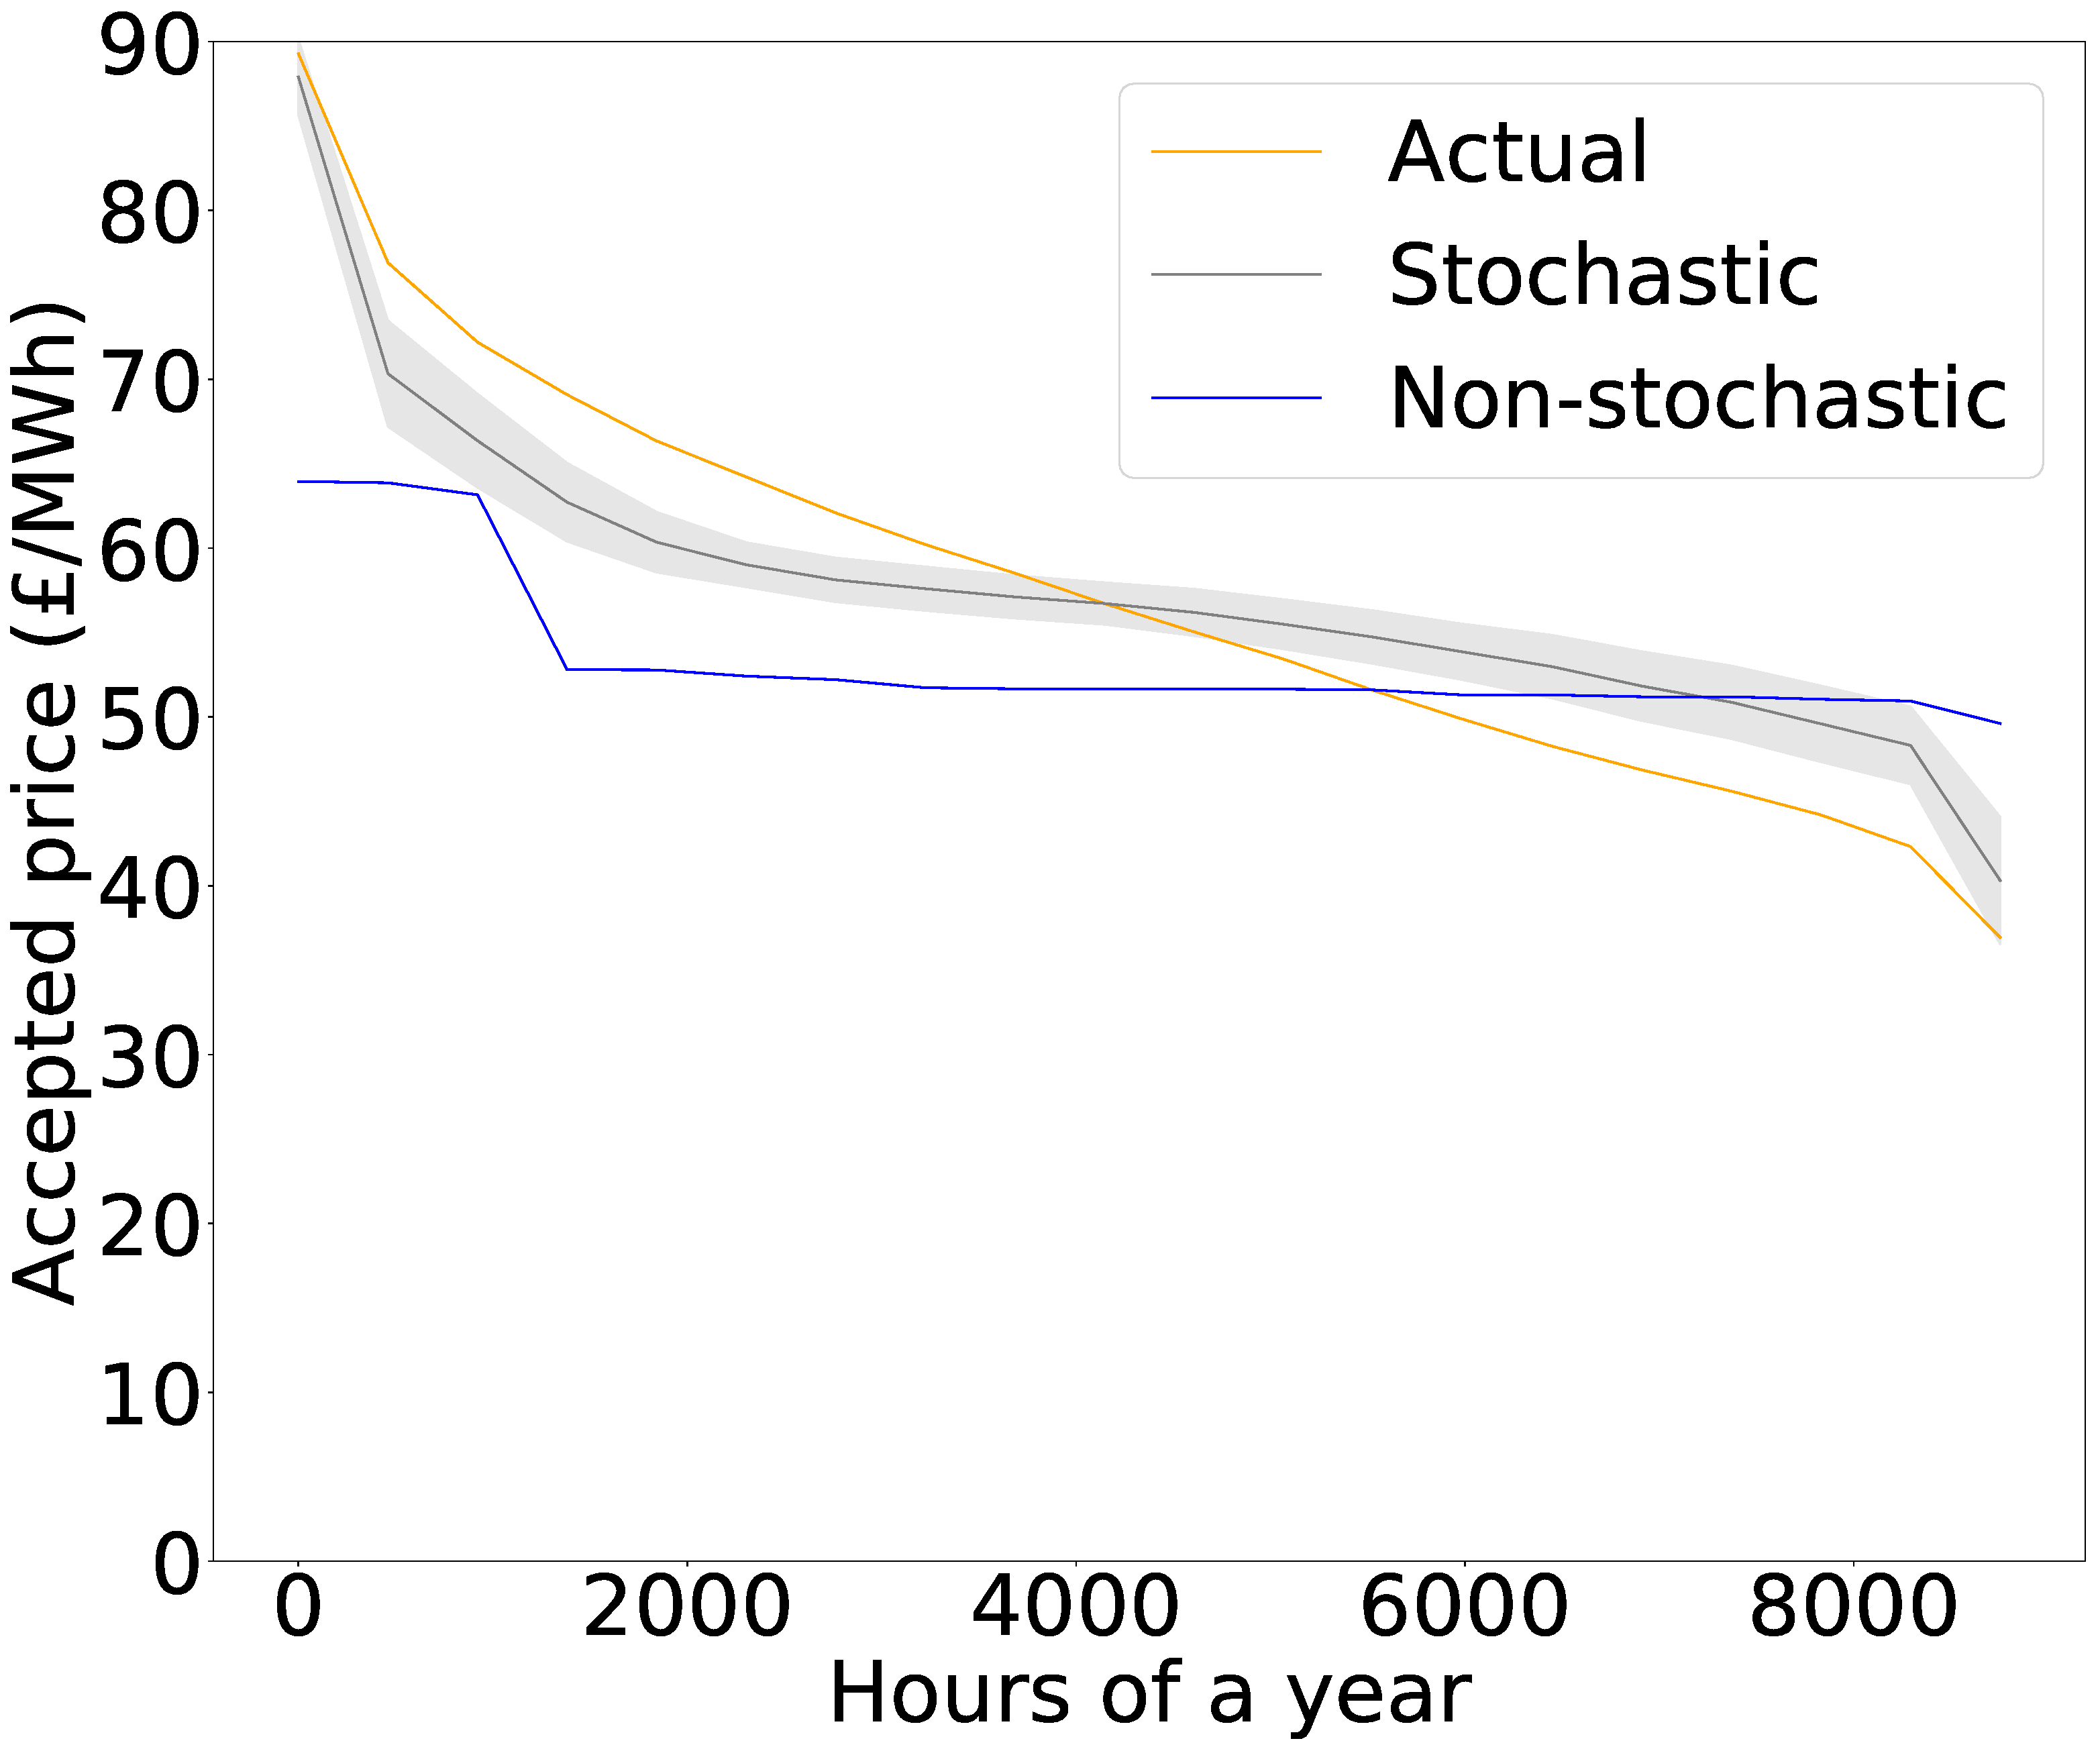
\includegraphics[width=0.35\textwidth]{figures/load_price_duration_curve_comparison.pdf}
		\caption{Price duration curve which compares real electricity prices to those paid in ElecSIM with and without stochasticity (2018).}
		\label{fig:price_duration_curve}
	\end{center}
\end{figure}


We ran the initialisation of the model 40 times to capture the price variance. Outliers were removed as on a small number of occasions large jumps in prices at peak demand occurred which deviated from the mean. We did this, as although this does occur in real life, it occurs at a smaller fraction of the time than 5\% of the year (modelled LDC), therefore the results would be unreasonably skewed for the highest demand segment. 

Figure \ref{fig:price_duration_curve} demonstrates very little variance in the non-stochastic case. This is due to the fact that combined cycle gas turbines (CCGTs) set the spot price. These CCGTs have little variance between one another as they were calibrated using the same dataset. By adding stochasticity of fuel prices and operation and maintenance prices, a curve that more closely resembles the actual data occurs. The stochastic curve, however, does not perfectly fit the real data, which may be due to higher variance in fuel prices and historical differences in operation and maintenance costs between power plants. One method of improving this would be fitting the data used to parametrise to the curve.

Table \ref{table:validation_metrics} shows performance metrics of the stochastic and non-stochastic runs versus the actual price duration curve . The stochastic implementation, improves the mean absolute error (MAE) of the non-stochastic case by $52.5\%$.

%\addtolength{\textfloatsep}{-0.05in}


\begin{table}
	\centering
	\csvautobooktabular{tables/validation/initialisation_run_validation.csv}
	\caption{Validation performance metrics.}
	\label{table:validation_metrics}
\end{table}
%\addtolength{\textfloatsep}{-0.05in}

By observing the processes that emerge from the long-term scenarios, we can see that carbon price and investment in renewable generation are positively correlated, as would be expected.

The highest NPV calculations were for onshore wind and CCGT plants. This is realistic for the United Kingdom, where subsidies are required for other forms of generation such as coal and nuclear.

\subsection{Performance}

 We used Microsoft Azure Public Cloud. Utilising two virtual machines of 64 vCPU's each (D64 v3), which are built using Intel Broadwell E5-2673 v4 2.3GHz processors, and the Intel Haswell 2.4 GHz E5-2673 v3. They have a total of 256GB of memory and use a Linux operating system. The total disk size of ElecSIM is 5.8MB. The memory used for a 10 year run has a median of 57.1MB.


\begin{figure}
	\centering
	\includegraphics[width=0.9\linewidth]{figures/timing_plot}
	\caption{Run times of different sized countries.}
	\label{fig:timingplot}
\end{figure}

Figure \ref{fig:timingplot} shows the running time for ElecSIM with varying installed capacity. We run the simulation with varying carbon taxes between 0, 20, 40 and \textsterling70 per tonne of \ce{CO2}. We varied demand between 2GW and 320GW to see the effect of different sized countries on running time. The makeup of the electricity mix was achieve through stratified sampling of the UK electricity mix. The results show a linear time complexity.

%\begin{itemize}
%	\item Validation of model 
%	\begin{itemize}
%		\item Compare price duration curve
%		\item Compare power plant costs and NPV calculations
%		\item Look number of steps ahead to compare electricity mix and compare to actual (cross-validation)
%	\end{itemize} 
%	\item Performance metrics - Comparison with EMLab, PowerACE (15 minute run time)
%	\begin{itemize}
%		\item Memory, disk size, runtime
%		\item Increase in time complexity with additional data.
%	\end{itemize}
%\end{itemize}



\section{Scenario Testing}\label{Scenario Testing}

This section describes scenario runs using ElecSIM. Here, we vary the carbon tax and either grow or reduce total electricity demand. This was done to observe the effects of carbon tax policy on long-term investment.

ElecSIM was built using python, this enabled us to lower barriers to entry and allow for users to integrate state-of-the-art machine learning and statistical packages in future work. We used project mesa as an open source agent based modelling framework for its ease of use \cite{Masad2015}.

% {\color{blue}
% We assume that carbon tax is set by the government, and not subject to market forces such as the EU Emissions Trading Scheme \cite{Council2016}.

% We run 16 different scenarios 8 times each, with demand increasing and decreasing by 1\% per year and  varying carbon prices. In this section we explore a decreasing demand of 1\% a year. We chose this due to the increasing efficiency of homes, industry and technology, and due to the recent trend in the UK. Demand, however, did not display a large effect on the optimum carbon price. We select a burn-in period of 6 years, due to the fact that the majority of power plants take 6 years to go from investment to operation.

% Table \ref{table:scenario_statistics}, in the appendix, displays the summary statistics of each run.

% It can be seen from Figure \ref{fig:demand99carbon10} that a carbon tax of \textsterling10 per year does little to influence investment in low-carbon, renewable technology. With traditional, fossil fuel based generation, providing the majority of supply in each year. However, there is an increase in renewable technology over the years, starting from mean 15.85\% market share in the year range 2019-2029, to 24.38\% in the year range 2039-2050. A similar increase of renewable energy with a carbon tax of \textsterling0 can be seen, albeit at a lower mean by the year range 2039-2050 (22.29\%).
% }

The UK Government BEIS have predicted a carbon tax increasing from \textsterling18 to \textsterling200 by 2050. With carbon price increasingly linearly from 2030 to 2050. We have approximated these assumptions in Figure \ref{fig:demand99carbon18} and modelled the results. Interestingly, the results show only a slight increase in low-carbon supply over the \textsterling20 carbon tax energy mix. This demonstrates the importance of long-term modelling, and understanding the long-term impacts that can result due to today's decisions.

It is hypothesised that a lower carbon tax early on changes the market dynamics for years to come, due to certain price structures, and therefore it takes a long time for renewable energy to recover.

Figure \ref{fig:demand99carbon40} shows that a carbon tax of \textsterling40 is sufficient in beginning to move towards a low-carbon economy, with backup fossil fuel generators.

However, by referring to Figure \ref{fig:demand99carbon70} it can be seen that to have 100\% renewable, a carbon price of \textsterling70 is required. 

These results show the importance of making difficult decisions as soon as possible to have the biggest effect on the energy mix for years to come.

% \begin{figure}
	% \begin{center}
% 		\includegraphics[width=0.5\textwidth]{figures/scenarios/demand099-carbon70-datetime.png}
% 		\caption{{\color{blue}Demand decreasing by 1\% per year with a carbon tax of \textsterling70.}}
% 		\label{fig:demand99carbon70}
% 	\end{center}
% \end{figure}



 \begin{figure*}[h]
% 	\centering
% 	\begin{subfigure}[b]{0.475\textwidth}
% 		\centering
% 		\includegraphics[width=\textwidth]{figures/scenarios/demand099-carbon10-datetime.png}
% 		\caption[Network2]%
% 		{{{\color{blue}{\small \textsterling10 carbon tax.}}}}
% 		\label{fig:demand99carbon10}
% 	\end{subfigure}
% 	\hfill
% 	\begin{subfigure}[b]{0.475\textwidth}  
% 		\centering 
% 		\includegraphics[width=\textwidth]{figures/scenarios/demand099-carbon20-datetime.png}
% 		\caption[]%
% 		{{{\color{blue}\textsterling20 carbon tax.}}}
% 		\label{fig:demand99carbon20}
% 	\end{subfigure}
% 	\vskip\baselineskip


	\begin{subfigure}[b]{0.475\textwidth}   
		\centering 
		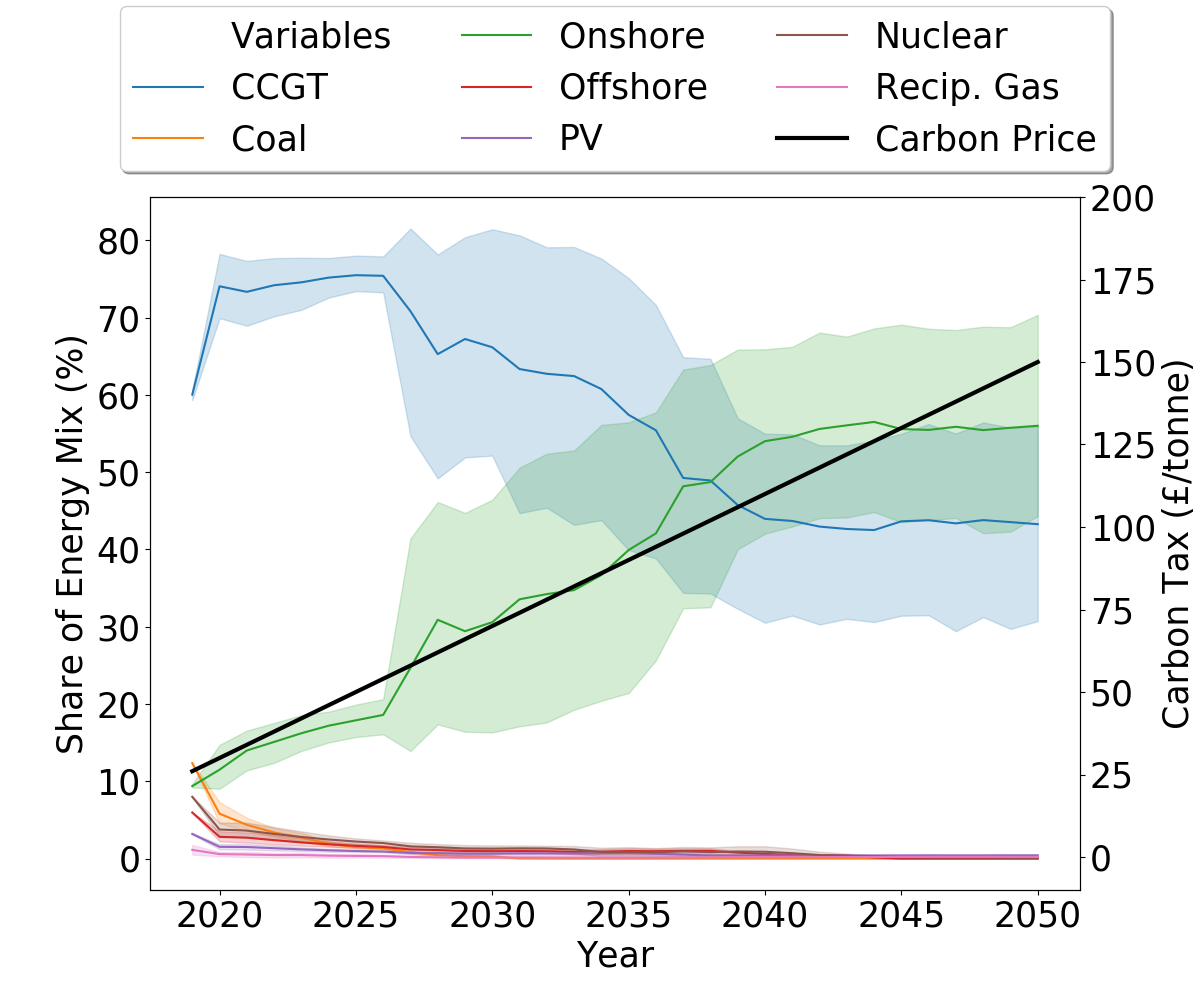
\includegraphics[width=\textwidth]{figures/scenarios/demand099-carbon18-datetime.png}
		\caption[]%
		{{\textsterling26 to \textsterling150 linearly increasing carbon tax.}}    
		\label{fig:demand99carbon18}
	\end{subfigure}
	\quad
	\begin{subfigure}[b]{0.475\textwidth}   
		\centering 
		\includegraphics[width=\textwidth]{figures/scenarios/demand099-carbon40-datetime.png}
		\caption[]%
		{{\textsterling40 carbon tax.}}    
		\label{fig:demand99carbon40}
	\end{subfigure}
	\caption[ Scenarios up to the year 2050 with varying carbon taxes and decreasing demand ]
	{\small Scenarios up to the year 2050, with varying carbon taxes and electricity demand decreasing 1\% a year.} 
	\label{fig:mean and std of nets}
\end{figure*}
%\FloatBarrier








%\begin{figure}[h]
%	\begin{center}
%		\includegraphics[width=0.5\textwidth]{figures/scenarios/demand099-carbon10-datetime.png}
%		\caption{Demand decreasing by 1\% per year and a carbon tax of \textsterling10}
%		\label{fig:demand99carbon10}
%	\end{center}
%\end{figure}
%
%\begin{figure}[h]
%	\begin{center}
%		\includegraphics[width=0.5\textwidth]{figures/scenarios/demand099-carbon20-datetime.png}
%		\caption{Demand decreasing by 1\% per year and a carbon tax of \textsterling20}
%		\label{fig:demand99carbon10}
%	\end{center}
%\end{figure}
%
%
%
%\begin{figure}[h]
%	\begin{center}
%		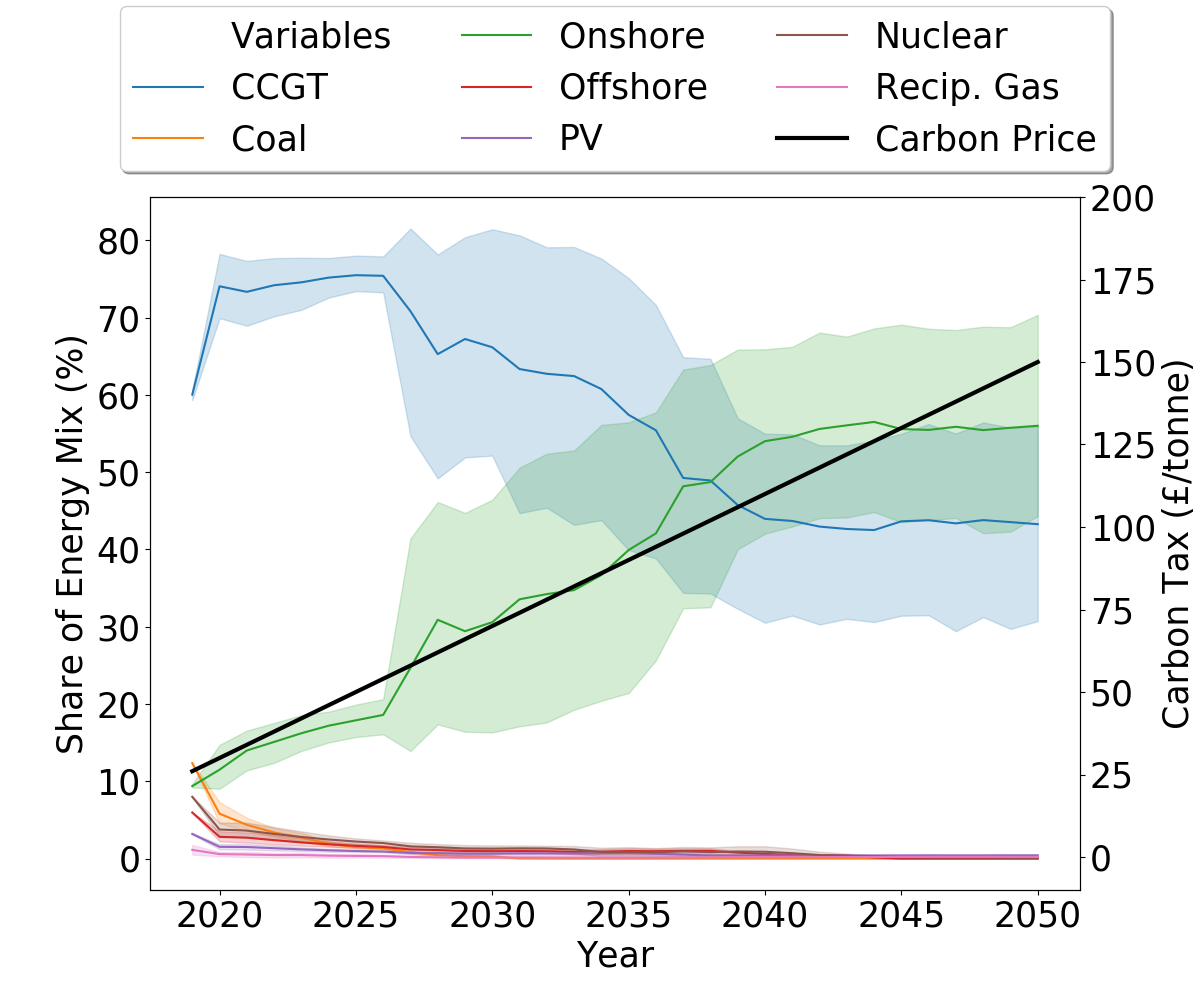
\includegraphics[width=0.5\textwidth]{figures/scenarios/demand099-carbon18-datetime.png}
%		\caption{Demand decreasing by 1\% per year and a carbon tax of \textsterling20}
%		\label{fig:demand99carbon10}
%	\end{center}
%\end{figure}
%
%
%
%\begin{figure}[h]
%	\begin{center}
%		\includegraphics[width=0.5\textwidth]{figures/scenarios/demand099-carbon40-datetime.png}
%		\caption{Demand decreasing by 1\% per year and a carbon tax of \textsterling20}
%		\label{fig:demand99carbon10}
%	\end{center}
%\end{figure}











%\begin{itemize}
%	\item Effect of different carbon tax on investments made.
%	\item Effects of different demand scenarios. (High peaks, high growth, high reduction in demand)
%	\item Effects of high fuel prices.
%	\item Different costs of capital (eg. Borrowing for Nuclear of interest rate to equal 2\% at government bonds rate, as opposed to 10\% for private companies.)
%	\item Different learning rates for renewable costs.
%	\item The effect of long term carbon tax policy (eg. Carbon price known for next 25 years) vs short term changes in carbon tax.
%\end{itemize}




\section{Conclusions}\label{Conclusion}


The fact that we have a liberalised electricity market with many heterogenous players means that ABMs are suited for modelling these electricity markets.

ABMs are able to model imperfect information as well as heterogeneous actors. ElecSIM models imperfect information through forecasting of electricity demand and future fuel and electricity prices. This leads to agents taking risk on their investments, and more realistically model market conditions.

We demonstrated that increasing carbon tax can lead to an increase in investment of low-carbon technologies. We showed that early decisions have a long-term impact on the energy mix. 

Our future work includes comparing agent-learning techniques, using multi-agent reinforcement learning algorithms and artificial intelligence to allow agents to learn in a non-static environment. We propose the integration of a higher temporal and spatial resolution to model changes in daily demand, as well as capacity factors by region, and transmission effects.

%\begin{itemize}
%	\item Requirement for agent based models based on imperfect information, liberalised energy markets
%	\item Requirement for low barriers to entry open source model.
%	\item Discuss results
%	\item Future work:
%	\begin{itemize}
%		\item Embedding multi-agent intelligence such as Genetic Algorithms,  Q-learning and dynamic reinforcement learning
%		\item Raise spatial and temporal resolution.
%	\end{itemize}
%\end{itemize}

\FloatBarrier




%
% The acknowledgments section is defined using the "acks" environment (and NOT an unnumbered section). This ensures
% the proper identification of the section in the article metadata, and the consistent spelling of the heading.


%\begin{acks}
%This work was supported by the Engineering and Physical Sciences Research Council, Centre for Doctoral Training in Cloud Computing for Big Data [grant number EP/L015358/1].
%\end{acks}


%
% The next two lines define the bibliography style to be used, and the bibliography file.
\bibliographystyle{ACM-Reference-Format}
\bibliography{library,custombibtex}

% 
% If your work has an appendix, this is the place to put it.
\appendix


\section{Research Methods}


Table \ref{table:modern_plant_costs} shows a sample of modern power plant costs, and Table \ref{table:historic_plant_costs} displays a sample of historic power plant costs. The parameters for both of these tables are explained in Section \ref{ssssec:powerplantparameters}

Table \ref{table:scenario_statistics} displays summary statistics for each scenario run. It demonstrates the demand and whether it increases or decreases and by the percentage of change. Carbon tax price in \textsterling\ per tonne of \ce{CO2}. Year range in which the summary statistics apply. 

We then split the low carbon and traditional generation into two groups. Traditional generation contains gas, coal and nuclear power plants, whereas the low carbon group contains photovoltaic as well as offshore and onshore wind turbines. "mean" stands for the arithmetic mean, "std" stands for standard deviation, and min and max are the minimum and maximum values respectively.

\subsection{Parameters}


\begin{table*}[]
	\begin{tabularx}{1.0205\linewidth}{|l|l|c|l|l|l|l|l|l|l|l|l|l|l|}
	\hline
	Type & Capacity & Year & $\eta$ & $OP$ & $P_D$ & $C_D$ & $P_C$ & $C_C$ & $I_C$ & $F_C$ & $V_C$ & $In_C$ & $Con_C$ \\ \hline
	\multirow{3}{*}{CCGT} & 168.0 & 2018/20/25 & 0.34 & 25 & 3 & 3 & 60,000 & 700,000 & 13,600 & 28,200 & 5 & 2,900 & 3,300 \\ \cline{2-14} 
	& 1200.0 & 2018/20/25 & 0.54 & 25 & 3 & 3 & 10,000 & 500,000 & 15,100 & 12,200 & 3 & 2,100 & 3,300 \\ \cline{2-14} 
	& 1471.0 & 2018/20/25 & 0.53 & 25 & 3 & 3 & 10,000 & 500,000 & 15,100 & 11,400 & 3 & 1,900 & 3,300 \\ \hline
	\multirow{5}{*}{Coal} & 552.0 & 2025 & 0.32 & 25 & 6 & 6 & 40,000 & 3,400,000 & 10,000 & 68,200 & 6 & 13,000 & 3,800 \\ \cline{2-14} 
	& 624.0 & 2025 & 0.32 & 25 & 5 & 5 & 70,000 & 4,200,000 & 10,000 & 79,600 & 3 & 19,300 & 3,800 \\ \cline{2-14} 
	& 652.0 & 2025 & 0.3 & 25 & 5 & 5 & 60,000 & 3,900,000 & 10,000 & 65,300 & 5 & 22,700 & 3,800 \\ \cline{2-14} 
	& 734.0 & 2025 & 0.38 & 25 & 5 & 5 & 60,000 & 2,600,000 & 10,000 & 56,400 & 3 & 9,600 & 3,800 \\ \cline{2-14} 
	& 760.0 & 2025 & 0.35 & 25 & 5 & 5 & 40,000 & 2,800,000 & 10,000 & 52,100 & 5 & 14,000 & 3,800 \\ \hline
	\multirow{3}{*}{Hydro} & 0.033 & 2018/20/25 & 1.0 & 35 & 0 & 0 & 0 & 6,300,000 & 0 & 83,300 & 0 & 0 & 0 \\ \cline{2-14} 
	& 1.046 & 2018/20/25 & 1.0 & 35 & 0 & 0 & 0 & 3,300,000 & 400 & 18,200 & 0 & 0 & 0 \\ \cline{2-14} 
	& 11.0 & 2018/20/25 & 1.0 & 41 & 2 & 2 & 60,000 & 3,000,000 & 0 & 45,100 & 6 & 0 & 0 \\ \hline
	Nuclear & 3300.0 & 2025 & 1.0 & 60 & 5 & 8 & 240,000 & 4,100,000 & 11,500 & 72,900 & 5 & 10,000 & 500 \\ \hline
	\multirow{5}{*}{OCGT} & 96.0 & 2018/20/25 & 0.35 & 25 & 2 & 2 & 80,000 & 600,000 & 12,600 & 9,900 & 4 & 2,500 & 2,400 \\ \cline{2-14} 
	& 299.0 & 2018/20/25 & 0.35 & 25 & 2 & 2 & 30,000 & 400,000 & 13,600 & 9,600 & 3 & 1,600 & 2,500 \\ \cline{2-14} 
	& 311.0 & 2018/20/25 & 0.35 & 25 & 2 & 2 & 30,000 & 400,000 & 13,600 & 9,500 & 3 & 1,600 & 2,500 \\ \cline{2-14} 
	& 400.0 & 2018/20/25 & 0.34 & 25 & 2 & 2 & 30,000 & 300,000 & 15,100 & 7,800 & 3 & 1,300 & 2,500 \\ \cline{2-14} 
	& 625.0 & 2018/20/25 & 0.35 & 25 & 2 & 2 & 20,000 & 300,000 & 15,100 & 4,600 & 3 & 1,200 & 2,400 \\ \hline
	\multirow{6}{*}{Offshore} & \multirow{3}{*}{321.0} & 2018 & 0.0 & 23 & 5 & 3 & 60,000 & 2,200,000 & 69,300 & 30,900 & 3 & 1,400 & 33,500 \\ \cline{3-14} 
	&  & 2020 & 0.0 & 23 & 5 & 3 & 60,000 & 2,100,000 & 69,300 & 30,000 & 3 & 1,400 & 32,600 \\ \cline{3-14} 
	&  & 2025 & 0.0 & 23 & 5 & 3 & 60,000 & 1,900,000 & 69,300 & 28,600 & 3 & 1,300 & 31,100 \\ \cline{2-14} 
	& \multirow{3}{*}{844.0} & 2018 & 0.0 & 22 & 5 & 3 & 120,000 & 2,400,000 & 323,000 & 48,600 & 4 & 3,300 & 50,300 \\ \cline{3-14} 
	&  & 2020 & 0.0 & 22 & 5 & 3 & 120,000 & 2,300,000 & 323,000 & 47,300 & 3 & 3,300 & 48,900 \\ \cline{3-14} 
	&  & 2025 & 0.0 & 22 & 5 & 3 & 120,000 & 2,100,000 & 323,000 & 45,400 & 3 & 3,100 & 47,000 \\ \hline
	\multirow{9}{*}{Onshore} & \multirow{3}{*}{0.01} & 2018 & 1.0 & 20 & 0 & 0 & 0 & 3,700,000 & 0 & 29,700 & 0 & 0 & 0 \\ \cline{3-14} 
	&  & 2020 & 1.0 & 20 & 0 & 0 & 0 & 3,600,000 & 0 & 29,600 & 0 & 0 & 0 \\ \cline{3-14} 
	&  & 2025 & 1.0 & 20 & 0 & 0 & 0 & 3,500,000 & 0 & 29,600 & 0 & 0 & 0 \\ \cline{2-14} 
	& \multirow{3}{*}{0.482} & 2018 & 1.0 & 20 & 0 & 0 & 0 & 2,200,000 & 200 & 56,900 & 0 & 0 & 0 \\ \cline{3-14} 
	&  & 2020 & 1.0 & 20 & 0 & 0 & 0 & 2,100,000 & 200 & 56,900 & 0 & 0 & 0 \\ \cline{3-14} 
	&  & 2025 & 1.0 & 20 & 0 & 0 & 0 & 2,000,000 & 200 & 56,700 & 0 & 0 & 0 \\ \cline{2-14} 
	& \multirow{3}{*}{20.0} & 2018 & 0.0 & 24 & 4 & 2 & 110,000 & 1,200,000 & 3,300 & 23,200 & 5 & 1,400 & 3,100 \\ \cline{3-14} 
	&  & 2020 & 0.0 & 24 & 4 & 2 & 110,000 & 1,200,000 & 3,300 & 23,000 & 5 & 1,400 & 3,100 \\ \cline{3-14} 
	&  & 2025 & 0.0 & 24 & 4 & 2 & 110,000 & 1,200,000 & 3,300 & 22,400 & 5 & 1,400 & 3,000 \\ \hline
	\multirow{14}{*}{PV} & \multirow{3}{*}{0.003} & 2018 & 1.0 & 30 & 0 & 0 & 0 & 1,500,000 & 0 & 23,500 & 0 & 0 & 0 \\ \cline{3-14} 
	&  & 2020 & 1.0 & 30 & 0 & 0 & 0 & 1,500,000 & 0 & 23,400 & 0 & 0 & 0 \\ \cline{3-14} 
	&  & 2025 & 1.0 & 30 & 0 & 0 & 0 & 1,400,000 & 0 & 23,200 & 0 & 0 & 0 \\ \cline{2-14} 
	& \multirow{2}{*}{0.455} & 2018 & 1.0 & 30 & 0 & 0 & 0 & 1,000,000 & 200 & 9,400 & 0 & 0 & 0 \\ \cline{3-14} 
	&  & 2025 & 1.0 & 30 & 0 & 0 & 0 & 900,000 & 200 & 9,200 & 0 & 0 & 0 \\ \cline{2-14} 
	& \multirow{3}{*}{1.0} & 2018 & 0.0 & 25 & 1 & 0 & 20,000 & 700,000 & 0 & 6,600 & 3 & 2,600 & 1,300 \\ \cline{3-14} 
	&  & 2020 & 0.0 & 25 & 1 & 0 & 20,000 & 700,000 & 0 & 6,300 & 3 & 2,600 & 1,300 \\ \cline{3-14} 
	&  & 2025 & 0.0 & 25 & 1 & 0 & 20,000 & 600,000 & 0 & 5,900 & 3 & 2,400 & 1,200 \\ \cline{2-14} 
	& \multirow{3}{*}{4.0} & 2018 & 0.0 & 25 & 1 & 0 & 60,000 & 700,000 & 200 & 8,300 & 0 & 1,200 & 1,300 \\ \cline{3-14} 
	&  & 2020 & 0.0 & 25 & 1 & 0 & 60,000 & 700,000 & 200 & 8,000 & 0 & 1,100 & 1,300 \\ \cline{3-14} 
	&  & 2025 & 0.0 & 25 & 1 & 0 & 60,000 & 600,000 & 200 & 7,500 & 0 & 1,100 & 1,200 \\ \cline{2-14} 
	& \multirow{3}{*}{16.0} & 2018 & 0.0 & 25 & 1 & 0 & 70,000 & 700,000 & 400 & 5,600 & 0 & 2,000 & 1,300 \\ \cline{3-14} 
	&  & 2020 & 0.0 & 25 & 1 & 0 & 70,000 & 600,000 & 400 & 5,400 & 0 & 1,900 & 1,300 \\ \cline{3-14} 
	&  & 2025 & 0.0 & 25 & 1 & 0 & 70,000 & 600,000 & 400 & 5,100 & 0 & 1,800 & 1,200 \\ \hline
	Recip. Engine (Diesel) & 20.0 & 2018/20/25 & 0.34 & 15 & 2 & 1 & 10,000 & 300,000 & 2,200 & 10,000 & 2 & 1,000 & -31,900 \\ \hline
	Recip. Engine (Gas) & 20.0 & 2018/20/25 & 0.32 & 15 & 2 & 1 & 10,000 & 300,000 & 3,400 & 10,000 & 2 & 1,000 & -31,900 \\ \hline
		
	\end{tabularx}
	

	\caption{Modern power plant costs \cite{Department2016}}
	\label{table:modern_plant_costs}
\end{table*}


% Please add the following required packages to your document preamble:
% \usepackage{multirow}
\begin{table*}[]
	\begin{tabular}{|l|l|l|l|l|l|l|l|l|l|l|l|l|l|}
	\hline
	Type & Capacity & Year & $\eta$ & $OP$ & $P_D$ & $C_D$ & $P_C$ & $C_C$ & $I_C$ & $F_C$ & $V_C$ & $In_C$ & $Con_C$ \\ \hline
	\multirow{12}{*}{CCGT} & \multirow{4}{*}{168.0} & 1980 & 0.34 & 25 & 3 & 3 & 207,345 & 2,419,027 & 46,998 & 97,452 & 22 & 10,021 & 11,403 \\ \cline{3-14} 
	&  & 1990 & 0.34 & 25 & 3 & 3 & 181,208 & 2,114,099 & 41,073 & 85,167 & 13 & 8,758 & 9,966 \\ \cline{3-14} 
	&  & 2000 & 0.34 & 25 & 3 & 3 & 116,407 & 1,358,089 & 26,385 & 54,711 & 10 & 5,626 & 6,402 \\ \cline{3-14} 
	&  & 2010 & 0.34 & 25 & 3 & 3 & 73,530 & 857,857 & 16,666 & 34,559 & 11 & 3,553 & 4,044 \\ \cline{2-14} 
	& \multirow{4}{*}{1200.0} & 1980 & 0.54 & 25 & 3 & 3 & 59,102 & 2,955,138 & 89,245 & 72,105 & 31 & 12,411 & 19,503 \\ \cline{3-14} 
	&  & 1990 & 0.54 & 25 & 3 & 3 & 59,884 & 2,994,246 & 90,426 & 73,059 & 21 & 12,575 & 19,762 \\ \cline{3-14} 
	&  & 2000 & 0.54 & 25 & 3 & 3 & 49,674 & 2,483,747 & 75,009 & 60,603 & 21 & 10,431 & 16,392 \\ \cline{3-14} 
	&  & 2010 & 0.54 & 25 & 3 & 3 & 60,640 & 3,032,008 & 91,566 & 73,981 & 13 & 12,734 & 20,011 \\ \cline{2-14} 
	& \multirow{4}{*}{1471.0} & 1980 & 0.53 & 25 & 3 & 3 & 92,000 & 4,600,023 & 138,920 & 104,880 & 10 & 17,480 & 30,360 \\ \cline{3-14} 
	&  & 1990 & 0.53 & 25 & 3 & 3 & 54,296 & 2,714,817 & 81,987 & 61,897 & 26 & 10,316 & 17,917 \\ \cline{3-14} 
	&  & 2000 & 0.53 & 25 & 3 & 3 & 49,310 & 2,465,515 & 74,458 & 56,213 & 21 & 9,368 & 16,272 \\ \cline{3-14} 
	&  & 2010 & 0.53 & 25 & 3 & 3 & 46,998 & 2,349,947 & 70,968 & 53,578 & 21 & 8,929 & 15,509 \\ \hline
	\multirow{24}{*}{Coal} & \multirow{4}{*}{552.0} & 1980 & 0.32 & 25 & 6 & 6 & 118,041 & 10,033,488 & 29,510 & 201,259 & 22 & 38,363 & 11,213 \\ \cline{3-14} 
	&  & 1990 & 0.32 & 25 & 6 & 6 & 41,766 & 3,550,192 & 10,441 & 71,212 & 2 & 13,574 & 3,967 \\ \cline{3-14} 
	&  & 2000 & 0.32 & 25 & 6 & 6 & 51,429 & 4,371,538 & 12,857 & 87,687 & 3 & 16,714 & 4,885 \\ \cline{3-14} 
	&  & 2010 & 0.32 & 25 & 6 & 6 & 43,411 & 3,689,957 & 10,852 & 74,016 & 10 & 14,108 & 4,124 \\ \cline{2-14} 
	& \multirow{8}{*}{624.0} & 1980 & 0.32 & 25 & 5 & 5 & 183,851 & 11,031,076 & 26,264 & 206,176 & 15 & 41,497 & 9,980 \\ \cline{3-14} 
	&  & 1980 & 0.32 & 25 & 5 & 5 & 188,476 & 11,308,571 & 26,925 & 211,362 & 11 & 42,541 & 10,231 \\ \cline{3-14} 
	&  & 1990 & 0.32 & 25 & 5 & 5 & 62,458 & 3,747,483 & 8,922 & 70,042 & 5 & 14,097 & 3,390 \\ \cline{3-14} 
	&  & 1990 & 0.32 & 25 & 5 & 5 & 65,126 & 3,907,588 & 9,303 & 73,034 & 3 & 14,699 & 3,535 \\ \cline{3-14} 
	&  & 2000 & 0.32 & 25 & 5 & 5 & 80,033 & 4,802,002 & 11,433 & 89,751 & 3 & 18,064 & 4,344 \\ \cline{3-14} 
	&  & 2000 & 0.32 & 25 & 5 & 5 & 80,882 & 4,852,979 & 11,554 & 90,704 & 3 & 18,256 & 4,390 \\ \cline{3-14} 
	&  & 2010 & 0.32 & 25 & 5 & 5 & 84,549 & 5,072,973 & 12,078 & 94,816 & 3 & 19,084 & 4,589 \\ \cline{3-14} 
	&  & 2010 & 0.32 & 25 & 5 & 5 & 81,834 & 4,910,056 & 11,690 & 91,771 & 5 & 18,471 & 4,442 \\ \cline{2-14} 
	& \multirow{4}{*}{652.0} & 1980 & 0.3 & 25 & 5 & 5 & 161,344 & 10,487,387 & 26,890 & 175,596 & 16 & 61,041 & 10,218 \\ \cline{3-14} 
	&  & 1990 & 0.3 & 25 & 5 & 5 & 54,542 & 3,545,235 & 9,090 & 59,359 & 4 & 20,635 & 3,454 \\ \cline{3-14} 
	&  & 2000 & 0.3 & 25 & 5 & 5 & 68,516 & 4,453,581 & 11,419 & 74,568 & 2 & 25,922 & 4,339 \\ \cline{3-14} 
	&  & 2010 & 0.3 & 25 & 5 & 5 & 67,915 & 4,414,497 & 11,319 & 73,914 & 4 & 25,694 & 4,301 \\ \cline{2-14} 
	& \multirow{4}{*}{734.0} & 1980 & 0.38 & 25 & 5 & 5 & 249,766 & 10,823,198 & 41,627 & 234,780 & 16 & 39,962 & 15,818 \\ \cline{3-14} 
	&  & 1990 & 0.38 & 25 & 5 & 5 & 87,920 & 3,809,903 & 14,653 & 82,645 & 7 & 14,067 & 5,568 \\ \cline{3-14} 
	&  & 2000 & 0.38 & 25 & 5 & 5 & 118,072 & 5,116,482 & 19,678 & 110,988 & 5 & 18,891 & 7,477 \\ \cline{3-14} 
	&  & 2010 & 0.38 & 25 & 5 & 5 & 132,370 & 5,736,075 & 22,061 & 124,428 & 5 & 21,179 & 8,383 \\ \cline{2-14} 
	& \multirow{4}{*}{760.0} & 1980 & 0.35 & 25 & 5 & 5 & 160,182 & 11,212,746 & 40,045 & 208,637 & 8 & 56,063 & 15,217 \\ \cline{3-14} 
	&  & 1990 & 0.35 & 25 & 5 & 5 & 55,208 & 3,864,573 & 13,802 & 71,908 & 4 & 19,322 & 5,244 \\ \cline{3-14} 
	&  & 2000 & 0.35 & 25 & 5 & 5 & 65,705 & 4,599,358 & 16,426 & 85,580 & 8 & 22,996 & 6,241 \\ \cline{3-14} 
	&  & 2010 & 0.35 & 25 & 5 & 5 & 77,393 & 5,417,570 & 19,348 & 100,805 & 3 & 27,087 & 7,352 \\ \hline
	\multirow{4}{*}{Nuclear} & \multirow{4}{*}{3300.0} & 1980 & 1.0 & 60 & 5 & 8 & 516,790 & 8,828,507 & 24,762 & 156,975 & 21 & 21,532 & 1,076 \\ \cline{3-14} 
	&  & 1990 & 1.0 & 60 & 5 & 8 & 390,159 & 6,665,224 & 18,695 & 118,510 & 3 & 16,256 & 812 \\ \cline{3-14} 
	&  & 2000 & 1.0 & 60 & 5 & 8 & 378,998 & 6,474,560 & 18,160 & 115,120 & 15 & 15,791 & 789 \\ \cline{3-14} 
	&  & 2010 & 1.0 & 60 & 5 & 8 & 388,457 & 6,636,156 & 18,613 & 117,994 & 13 & 16,185 & 809 \\ \hline
	\multirow{8}{*}{Offshore} & \multirow{4}{*}{321.0} & 1980 & 0.0 & 23 & 5 & 3 & 100,043 & 3,668,254 & 115,550 & 51,522 & 9 & 2,334 & 55,857 \\ \cline{3-14} 
	&  & 1990 & 0.0 & 23 & 5 & 3 & 104,550 & 3,833,513 & 120,755 & 53,843 & 3 & 2,439 & 58,373 \\ \cline{3-14} 
	&  & 2000 & 0.0 & 23 & 5 & 3 & 102,374 & 3,753,742 & 118,242 & 52,723 & 6 & 2,388 & 57,159 \\ \cline{3-14} 
	&  & 2010 & 0.0 & 23 & 5 & 3 & 98,571 & 3,614,292 & 113,850 & 50,764 & 6 & 2,300 & 55,035 \\ \cline{2-14} 
	& \multirow{4}{*}{844.0} & 1980 & 0.0 & 22 & 5 & 3 & 181,469 & 3,629,393 & 488,455 & 73,495 & 8 & 4,990 & 76,066 \\ \cline{3-14} 
	&  & 1990 & 0.0 & 22 & 5 & 3 & 178,822 & 3,576,447 & 481,330 & 72,423 & 10 & 4,917 & 74,956 \\ \cline{3-14} 
	&  & 2000 & 0.0 & 22 & 5 & 3 & 180,212 & 3,604,250 & 485,072 & 72,986 & 9 & 4,955 & 75,539 \\ \cline{3-14} 
	&  & 2010 & 0.0 & 22 & 5 & 3 & 171,372 & 3,427,446 & 461,277 & 69,405 & 11 & 4,712 & 71,833 \\ \hline
	\multirow{4}{*}{Onshore} & \multirow{4}{*}{20.0} & 1980 & 0.0 & 24 & 4 & 2 & 374,087 & 4,080,950 & 11,222 & 78,898 & 26 & 4,761 & 10,542 \\ \cline{3-14} 
	&  & 1990 & 0.0 & 24 & 4 & 2 & 411,234 & 4,486,197 & 12,337 & 86,733 & 10 & 5,233 & 11,589 \\ \cline{3-14} 
	&  & 2000 & 0.0 & 24 & 4 & 2 & 230,491 & 2,514,457 & 6,914 & 48,612 & 5 & 2,933 & 6,495 \\ \cline{3-14} 
	&  & 2010 & 0.0 & 24 & 4 & 2 & 143,450 & 1,564,915 & 4,303 & 30,255 & 7 & 1,825 & 4,042 \\ \hline
	\multirow{4}{*}{PV} & \multirow{4}{*}{16.0} & 1980 & 0.0 & 25 & 1 & 0 & 399,799 & 3,997,991 & 2,284 & 31,983 & 0 & 11,422 & 7,424 \\ \cline{3-14} 
	&  & 1990 & 0.0 & 25 & 1 & 0 & 399,799 & 3,997,991 & 2,284 & 31,983 & 0 & 11,422 & 7,424 \\ \cline{3-14} 
	&  & 2000 & 0.0 & 25 & 1 & 0 & 399,799 & 3,997,991 & 2,284 & 31,983 & 0 & 11,422 & 7,424 \\ \cline{3-14} 
	&  & 2010 & 0.0 & 25 & 1 & 0 & 399,799 & 3,997,991 & 2,284 & 31,983 & 0 & 11,422 & 7,424 \\ \hline
	\end{tabular}
	\caption{Sample of historic power plant costs \cite{IRENA2018,IEA2015,OWPB2016}} 
	\label{table:historic_plant_costs}

\end{table*}

\clearpage

%\subsection{Scenario Runs}

%\begin{table}[h]
%	\centering
%	\csvautobooktabular{tables/scenarios/demand90.csv}
%	\caption{Scenario Runs.}
%\end{table}






\begin{table*}[H]
	\begin{tabular}{|l|l|l|l|l|l|l|l|l|l|l|}
		\hline
		\multirow{2}{*}{\textbf{Demand}} & \multirow{2}{*}{\textbf{Carbon Tax}} & \multirow{2}{*}{\textbf{Year Range}} & \multicolumn{4}{l|}{\textbf{Low Carbon}} & \multicolumn{4}{l|}{\textbf{Traditional Generation}} \\ \cline{4-11} 
		&  &  & \textbf{mean} & \textbf{std} & \textbf{min} & \textbf{max} & \textbf{mean} & \textbf{std} & \textbf{min} & \textbf{max} \\ \hline
		\multirow{24}{*}{Demand Decreasing 1\% a Year} & \multirow{3}{*}{0} & 2019-2029 & 14.14 & 5.16 & 6.36 & 27.29 & 85.86 & 5.16 & 72.71 & 93.64 \\ \cline{3-11} 
		&  & 2029-2039 & 16.95 & 11.19 & 6.2 & 52.52 & 83.05 & 11.19 & 47.48 & 93.8 \\ \cline{3-11} 
		&  & 2039-2050 & 22.29 & 18.01 & 4.72 & 60.0 & 77.71 & 18.01 & 40.0 & 95.28 \\ \cline{2-11} 
		& \multirow{3}{*}{10} & 2019-2029 & 15.85 & 8.82 & 8.8 & 41.0 & 84.15 & 8.82 & 59.0 & 91.2 \\ \cline{3-11} 
		&  & 2029-2039 & 20.33 & 15.34 & 7.92 & 62.75 & 79.67 & 15.34 & 37.25 & 92.08 \\ \cline{3-11} 
		&  & 2039-2050 & 24.38 & 17.17 & 8.79 & 61.87 & 75.62 & 17.17 & 38.13 & 91.21 \\ \cline{2-11} 
		& \multirow{3}{*}{170 to 22} & 2019-2029 & 92.03 & 8.32 & 71.2 & 99.8 & 7.97 & 8.32 & 0.2 & 28.8 \\ \cline{3-11} 
		&  & 2029-2039 & 99.66 & 0.11 & 99.11 & 99.82 & 0.34 & 0.11 & 0.18 & 0.89 \\ \cline{3-11} 
		&  & 2039-2050 & 99.59 & 0.1 & 99.32 & 99.75 & 0.41 & 0.1 & 0.25 & 0.68 \\ \cline{2-11} 
		& \multirow{3}{*}{26 to 174} & 2019-2029 & 24.84 & 11.32 & 11.01 & 65.78 & 75.16 & 11.32 & 34.22 & 88.99 \\ \cline{3-11} 
		&  & 2029-2039 & 42.6 & 21.63 & 11.28 & 79.05 & 57.4 & 21.63 & 20.95 & 88.72 \\ \cline{3-11} 
		&  & 2039-2050 & 56.42 & 15.48 & 31.63 & 81.72 & 43.58 & 15.48 & 18.28 & 68.37 \\ \cline{2-11} 
		& \multirow{3}{*}{20} & 2019-2029 & 22.94 & 11.92 & 7.8 & 62.07 & 77.06 & 11.92 & 37.93 & 92.2 \\ \cline{3-11} 
		&  & 2029-2039 & 40.52 & 21.73 & 7.04 & 73.0 & 59.48 & 21.73 & 27.0 & 92.96 \\ \cline{3-11} 
		&  & 2039-2050 & 49.36 & 20.73 & 10.82 & 79.09 & 50.64 & 20.73 & 20.91 & 89.18 \\ \cline{2-11} 
		& \multirow{3}{*}{40} & 2019-2029 & 48.16 & 12.28 & 32.61 & 82.35 & 51.84 & 12.28 & 17.65 & 67.39 \\ \cline{3-11} 
		&  & 2029-2039 & 69.08 & 12.12 & 46.05 & 93.13 & 30.92 & 12.12 & 6.87 & 53.95 \\ \cline{3-11} 
		&  & 2039-2050 & 70.61 & 10.82 & 52.5 & 91.98 & 29.39 & 10.82 & 8.02 & 47.5 \\ \cline{2-11} 
		& \multirow{3}{*}{50} & 2019-2029 & 53.78 & 23.42 & 17.98 & 92.93 & 46.22 & 23.42 & 7.07 & 82.02 \\ \cline{3-11} 
		&  & 2029-2039 & 68.41 & 20.18 & 29.54 & 96.29 & 31.59 & 20.18 & 3.71 & 70.46 \\ \cline{3-11} 
		&  & 2039-2050 & 66.86 & 20.42 & 38.31 & 99.73 & 33.14 & 20.42 & 0.27 & 61.69 \\ \cline{2-11} 
		& \multirow{3}{*}{70} & 2019-2029 & 83.62 & 13.16 & 41.29 & 99.41 & 16.38 & 13.16 & 0.59 & 58.71 \\ \cline{3-11} 
		&  & 2029-2039 & 96.76 & 4.43 & 83.93 & 99.99 & 3.24 & 4.43 & 0.01 & 16.07 \\ \cline{3-11} 
		&  & 2039-2050 & 97.63 & 3.58 & 87.8 & 99.94 & 2.37 & 3.58 & 0.06 & 12.2 \\ \hline
		\multirow{24}{*}{Demand Increasing 1\% a Year} & \multirow{3}{*}{0} & 2019-2029 & 14.87 & 9.9 & 6.73 & 45.59 & 85.13 & 9.9 & 54.41 & 93.27 \\ \cline{3-11} 
		&  & 2029-2039 & 17.07 & 16.39 & 4.8 & 65.87 & 82.93 & 16.39 & 34.13 & 95.2 \\ \cline{3-11} 
		&  & 2039-2050 & 17.54 & 20.0 & 3.83 & 67.95 & 82.46 & 20.0 & 32.05 & 96.17 \\ \cline{2-11} 
		& \multirow{3}{*}{10} & 2019-2029 & 18.96 & 7.17 & 10.23 & 39.02 & 81.04 & 7.17 & 60.98 & 89.77 \\ \cline{3-11} 
		&  & 2029-2039 & 23.44 & 16.47 & 8.89 & 61.96 & 76.56 & 16.47 & 38.04 & 91.11 \\ \cline{3-11} 
		&  & 2039-2050 & 27.91 & 19.45 & 9.64 & 67.06 & 72.09 & 19.45 & 32.94 & 90.36 \\ \cline{2-11} 
		& \multirow{3}{*}{170 to 22} & 2019-2029 & 92.09 & 9.29 & 67.32 & 99.8 & 7.91 & 9.29 & 0.2 & 32.68 \\ \cline{3-11} 
		&  & 2029-2039 & 99.98 & 0.05 & 99.76 & 100.0 & 0.02 & 0.05 & 0.0 & 0.24 \\ \cline{3-11} 
		&  & 2039-2050 & 100.0 & 0.0 & 100.0 & 100.0 & 0.0 & 0.0 & 0.0 & 0.0 \\ \cline{2-11} 
		& \multirow{3}{*}{26 to 174} & 2019-2029 & 24.75 & 11.33 & 11.95 & 56.65 & 75.25 & 11.33 & 43.35 & 88.05 \\ \cline{3-11} 
		&  & 2029-2039 & 39.28 & 20.39 & 10.87 & 73.41 & 60.72 & 20.39 & 26.59 & 89.13 \\ \cline{3-11} 
		&  & 2039-2050 & 49.72 & 18.84 & 22.02 & 86.43 & 50.28 & 18.84 & 13.57 & 77.98 \\ \cline{2-11} 
		& \multirow{3}{*}{20} & 2019-2029 & 26.32 & 16.01 & 8.08 & 83.77 & 73.68 & 16.01 & 16.23 & 91.92 \\ \cline{3-11} 
		&  & 2029-2039 & 37.21 & 23.72 & 5.2 & 82.72 & 62.79 & 23.72 & 17.28 & 94.8 \\ \cline{3-11} 
		&  & 2039-2050 & 45.79 & 26.31 & 7.5 & 88.24 & 54.21 & 26.31 & 11.76 & 92.5 \\ \cline{2-11} 
		& \multirow{3}{*}{40} & 2019-2029 & 43.41 & 18.58 & 13.96 & 80.7 & 56.59 & 18.58 & 19.3 & 86.04 \\ \cline{3-11} 
		&  & 2029-2039 & 61.79 & 29.18 & 14.83 & 92.44 & 38.21 & 29.18 & 7.56 & 85.17 \\ \cline{3-11} 
		&  & 2039-2050 & 75.03 & 23.95 & 21.4 & 95.91 & 24.97 & 23.95 & 4.09 & 78.6 \\ \cline{2-11} 
		& \multirow{3}{*}{50} & 2019-2029 & 64.64 & 23.56 & 16.96 & 99.22 & 35.36 & 23.56 & 0.78 & 83.04 \\ \cline{3-11} 
		&  & 2029-2039 & 86.48 & 16.8 & 23.27 & 99.44 & 13.52 & 16.8 & 0.56 & 76.73 \\ \cline{3-11} 
		&  & 2039-2050 & 91.18 & 9.17 & 65.77 & 99.78 & 8.82 & 9.17 & 0.22 & 34.23 \\ \cline{2-11} 
		& \multirow{3}{*}{70} & 2019-2029 & 69.61 & 19.77 & 26.36 & 100.0 & 30.39 & 19.77 & 0.0 & 73.64 \\ \cline{3-11} 
		&  & 2029-2039 & 89.07 & 13.79 & 31.57 & 100.0 & 10.93 & 13.79 & 0.0 & 68.43 \\ \cline{3-11} 
		&  & 2039-2050 & 91.77 & 10.37 & 67.5 & 100.0 & 8.23 & 10.37 & 0.0 & 32.5 \\ \hline
	\end{tabular}
	\caption{Summary statistics for each scenario run.}
	\label{table:scenario_statistics} 
\end{table*}


\end{document}
